\PassOptionsToPackage{numbers}{natbib}
\documentclass{article}

\usepackage[final]{neurips_2024}

\usepackage[T1]{fontenc}
\usepackage[utf8]{inputenc}
\usepackage{xcolor}         % colors
\usepackage{hyperref}
\usepackage{url}
\usepackage{booktabs}
\usepackage{amsfonts}
\usepackage{amsmath}
\usepackage{amssymb}
\usepackage{graphicx}
\usepackage[section]{placeins}
\usepackage{microtype}
\usepackage{tabularx}
\usepackage{nicefrac}
\usepackage{multirow}
\usepackage[ruled]{algorithm2e}
\usepackage{listings}
\definecolor{codegreen}{rgb}{0.0,0.45,0.0}
\definecolor{codepurple}{rgb}{0.58,0.0,0.82}
\definecolor{codegray}{rgb}{0.45,0.45,0.45}
\lstset{
  language=Python,
  basicstyle=\ttfamily\small,
  keywordstyle=\color{blue},
  commentstyle=\color{codegreen}\itshape,
  stringstyle=\color{codepurple},
  numberstyle=\tiny\color{codegray},
  columns=fullflexible,
  keepspaces=true,
  breaklines=true,
  showstringspaces=false,
  frame=single,
  framerule=0.5pt,
  rulecolor=\color{black},
  framesep=5pt,
  aboveskip=0.6em,
  belowskip=0.6em
}
\SetInd{0.5em}{1.0em}
\renewcommand{\figurename}{Gambar}
\renewcommand{\tablename}{Tabel}
\renewcommand{\abstractname}{Abstrak}
\renewcommand{\refname}{Referensi}
\renewcommand{\algorithmcfname}{Algoritma}
\setlength{\textfloatsep}{10pt plus 2pt minus 2pt}
\setlength{\floatsep}{8pt plus 2pt minus 2pt}
\setlength{\intextsep}{8pt plus 2pt minus 2pt}
\renewcommand{\textfraction}{0.05}
\renewcommand{\floatpagefraction}{0.8}
\raggedbottom
\renewcommand{\theHfigure}{\thesection.\arabic{figure}}
\renewcommand{\theHtable}{\thesection.\arabic{table}}
\renewcommand{\theHalgocf}{\thesection.\arabic{algocf}}
\makeatletter
\renewcommand{\@noticestring}{Tugas Besar I Pembelajaran Mesin IF3270}
\makeatother

\title{FFNN untuk Prediksi Penempatan Kerja}

\author{%
Shanice Feodora Tjahjono \quad Muhammad Fathur Rizky \quad Ahmad Wicaksono \\
Kelompok \texttt{TorchIsAllYouNeed}, Program Studi Teknik Informatika, Institut Teknologi Bandung \\
\texttt{\{13523097,13523105,13523121\}@std.stei.itb.ac.id}
}

\begin{document}
\maketitle
\begin{center}
\vspace{-0.8em}
\includegraphics[width=0.45\linewidth]{logo.png}
\vspace{1.4em}
\end{center}

\begin{abstract}
Laporan ini membahas pembuatan \textit{feedforward neural network} (FFNN) dari awal dengan \texttt{NumPy} untuk memprediksi status penempatan kerja pada dataset \texttt{global\_student\_placement\_and\_salary}. Tujuan kami bukan hanya membuat model yang bisa dilatih, tetapi juga menyusun mini-framework yang cukup lengkap. Framework ini mencakup \textit{automatic differentiation} berbasis graph komputasi dinamis, abstraksi modul jaringan, fungsi aktivasi dan \textit{loss}, beberapa skema inisialisasi bobot, regularisasi L1/L2, optimizer \texttt{SGD} dan \texttt{Adam}, serta \texttt{RMSNorm}. Dari hasil eksperimen, terlihat bahwa performa model sangat dipengaruhi oleh kapasitas jaringan, inisialisasi, aktivasi, dan cara optimisasi yang dipakai. Konfigurasi terbaik pada studi kapasitas mencapai akurasi validasi 0.7520. Pada studi inisialisasi, \texttt{zero} tidak memberi titik awal pelatihan yang baik (akurasi 0.6155; \textit{validation loss} 0.666224), sedangkan Xavier memberi hasil terbaik di antara tiga skema yang diuji (\textit{validation loss} 0.488897). Penambahan \texttt{RMSNorm} juga menaikkan akurasi dari 0.7395 menjadi 0.7480 walaupun tidak selalu menurunkan \textit{loss}. Selain itu, implementasi kami juga lebih baik daripada baseline \texttt{sklearn MLPClassifier} pada setup yang sebanding (akurasi 0.7520 vs.\ 0.6975). Secara umum, hasil ini menunjukkan bahwa pilihan desain sistem dan detail implementasi numerik cukup berpengaruh terhadap stabilitas pelatihan dan kemampuan generalisasi model.
\end{abstract}

\section{Deskripsi Persoalan}
Dataset \texttt{global\_student\_placement\_and\_salary} berisi informasi akademik mahasiswa, pengalaman \textit{internship}, serta konteks institusi dan negara asal, dengan target \texttt{placement\_status}. Dalam laporan ini, persoalan tersebut dipandang sebagai klasifikasi biner: apakah seorang mahasiswa termasuk \textit{Placed} atau \textit{Not Placed}. Artinya, model harus mempelajari hubungan yang tidak selalu linear antara fitur-fitur numerik dan kategorikal, lalu mengubahnya menjadi probabilitas penempatan kerja.

\section{Pembahasan}
Implementasi pada proyek ini sengaja dibagi menjadi tiga lapisan utama. Lapisan pertama adalah \textit{autodiff core} pada kelas \texttt{Tensor} yang mengurus operasi diferensiabel dan aliran gradien. Lapisan kedua adalah abstraksi \texttt{nn.Module} yang menjadi dasar untuk komponen seperti layer, fungsi aktivasi, normalisasi, dan \textit{loss}. Lapisan ketiga adalah \texttt{optim} yang mengurus aturan update parameter. Pembagian ini membantu proses eksperimen karena arsitektur model bisa diubah, optimizer bisa diganti, dan fungsi aktivasi bisa dibandingkan tanpa harus mengubah mesin gradien utamanya. Susunan seperti ini juga sejalan dengan cara kerja sistem autodiff modern yang memisahkan graph diferensiasi, struktur model, dan proses optimisasi \citep{baydin2018ad,paszke2019pytorch}.

\section{Penjelasan Implementasi}
\subsection{Arsitektur Implementasi}
Arsitektur sistem dibangun di atas tiga lapisan yang saling melengkapi. Lapisan pertama adalah \textit{autodiff core} pada kelas \texttt{Tensor}. Di sini, satu objek menyimpan nilai numerik, gradien, parent pada graph komputasi, dan aturan turunan lokal. Lapisan kedua adalah abstraksi \texttt{Module} yang menjadi dasar untuk komponen model seperti \texttt{Linear}, \texttt{FFNN}, \texttt{Sequential}, kelas-kelas aktivasi, kelas-kelas \textit{loss}, dan \texttt{RMSNorm}. Lapisan ketiga adalah keluarga \texttt{Optimizer} yang memisahkan logika update parameter dari graph diferensiasi. Dengan pembagian seperti ini, tiap bagian punya tugas yang jelas dan perubahan pada satu bagian tidak langsung merusak bagian lain \citep{baydin2018ad,paszke2019pytorch}.

Dari sisi implementasi, susunan ini membuat alurnya lebih mudah diikuti. Data lebih dulu dibungkus menjadi \texttt{Tensor}, lalu diproses oleh rangkaian \texttt{Module}, menghasilkan \textit{loss} skalar, dan akhirnya parameternya diperbarui oleh \texttt{Optimizer}. Pada level model, \texttt{Linear} dipakai untuk operasi affine dasar, \texttt{Sequential} berperan sebagai kompositor modul umum, sedangkan \texttt{FFNN} menjadi pembungkus yang lebih praktis untuk eksperimen utama. Pada level data, \texttt{ArrayDataset} dan \texttt{DataLoader} menangani batching, pengacakan, dan reproduksibilitas eksperimen. Selain API berbasis kelas, sistem ini juga punya lapisan fungsional stateless untuk aktivasi dan \textit{loss} sehingga perhitungan numerik bisa diuji terpisah dari struktur model.

\noindent\textbf{Tiga mekanisme API utama}\par
Implementasi dibagi menjadi tiga mekanisme API. Mekanisme pertama adalah backend \texttt{Tensor} yang menangani operasi numerik dasar, perekaman graph, dan \texttt{backward()}. Mekanisme kedua adalah API layer \texttt{nn} yang berisi komponen stateful seperti \texttt{Linear}, \texttt{RMSNorm}, fungsi aktivasi, dan kelas-kelas \textit{loss}. Mekanisme ketiga adalah fungsi stateless pada namespace \texttt{torchlike.functional} yang dipakai untuk komputasi langsung berbasis NumPy atau \texttt{Tensor} ketika diperlukan validasi numerik atau komposisi yang lebih ringan.

Method \texttt{Module.parameters()} menjadi penghubung utama antara model dan proses optimisasi karena method ini mengumpulkan seluruh parameter trainable secara rekursif, termasuk yang tersimpan di dalam \texttt{list}, \texttt{tuple}, \texttt{dict}, atau submodule. Jadi, saat blok jaringan baru ditambahkan, pengembang cukup mendefinisikan atribut \texttt{Tensor(requires\_grad=True)} pada turunan \texttt{Module} dan parameternya akan ikut terdeteksi tanpa registrasi manual. Mekanisme ini sederhana tetapi penting karena menjadi dasar untuk pembahasan \textit{forward pass}, inisialisasi, aktivasi, \textit{loss}, autodiff, dan optimisasi.

\subsection{Struktur Kode Utama}
Bagian ini berfokus pada bentuk implementasi nyatanya. Setiap cuplikan kode diikuti penjelasan singkat agar pembaca bisa melihat dengan jelas bagaimana ide desain di bagian sebelumnya diterjemahkan menjadi kode.

\noindent\textbf{Kelas dasar \texttt{Module}}\par
\begin{lstlisting}
class Module:
    def forward(self, *args, **kwargs):
        raise NotImplementedError

    def __call__(self, *args, **kwargs):
        return self.forward(*args, **kwargs)

    def parameters(self):
        out, seen = [], set()
        for value in self.__dict__.values():
            self._collect_parameters(value, out, seen)
        return out
\end{lstlisting}
Kelas ini berfungsi sebagai kontrak dasar bagi semua komponen jaringan. Method \texttt{forward()} wajib diimplementasikan oleh kelas turunannya. Sementara itu, \texttt{parameters()} bertugas mengumpulkan semua \texttt{Tensor} trainable secara rekursif. Dengan desain seperti ini, optimizer tidak perlu mengetahui struktur internal model secara detail; ia cukup menerima daftar parameter yang sudah terkumpul.

\noindent\textbf{Alur reverse-mode pada \texttt{Tensor.backward}}\par
\begin{lstlisting}
def backward(self, grad=None):
    if grad is None:
        grad = np.ones_like(self.data)

    self.grad = self.grad + grad if self.grad is not None else grad
    topo, visited = [], set()

    def build(node):
        if id(node) in visited:
            return
        visited.add(id(node))
        for child in node._prev:
            build(child)
        topo.append(node)

    build(self)
    for node in reversed(topo):
        node._backward()
\end{lstlisting}
Implementasi autodiff memakai graph dinamis. Fungsi \texttt{build()} terlebih dahulu menyusun urutan topologis node-node yang relevan, lalu traversal terbalik menjalankan \textit{chain rule}. Setiap operasi tensor menyimpan aturan turunan lokalnya sendiri di \texttt{\_backward}. Karena itu, engine gradien tidak perlu mengetahui rumus khusus untuk seluruh model; ia cukup mengeksekusi aturan lokal setiap node secara berurutan.

\noindent\textbf{Layer \texttt{Linear}, \texttt{Sequential}, dan \texttt{FFNN}}\par
\begin{lstlisting}
class Linear(Module):
    def __init__(self, in_features, out_features, init="uniform", seed=None):
        self.weight = Tensor(_initialize((in_features, out_features), ...),
                             requires_grad=True)
        self.bias = Tensor(_initialize((1, out_features), ...),
                           requires_grad=True)

    def forward(self, x: Tensor) -> Tensor:
        return F.linear(x, self.weight, self.bias)

class Sequential(Module):
    def __init__(self, layers):
        self.layers = list(layers)

    def forward(self, x: Tensor) -> Tensor:
        out = x
        for layer in self.layers:
            out = layer(out)
        return out

class FFNN(Module):
    def __init__(self, layer_sizes, activations=None, init="uniform", seed=None):
        layers = []
        ...
        self.network = Sequential(layers)

    def forward(self, x: Tensor) -> Tensor:
        return self.network(x)
\end{lstlisting}
\texttt{Linear} menangani inisialisasi bobot sekaligus operasi affine dasar. \texttt{Sequential} mengatur alur eksekusi layer secara deklaratif dari awal sampai akhir. Di atasnya, \texttt{FFNN} menyusun beberapa layer linear dan aktivasi menjadi arsitektur yang siap dipakai di eksperimen. Jadi, pada notebook terbaru, sebagian besar studi memakai \texttt{FFNN} sebagai antarmuka utama, sedangkan \texttt{Sequential} tetap dipakai ketika susunan layer perlu dirakit lebih manual.

\noindent\textbf{Catatan transisi optimizer}\par
Implementasi detail update bobot sengaja dipusatkan pada Subbagian~\ref{subsec:optimizer} agar pembahasan tidak berulang. Bagian ini hanya memperlihatkan struktur model dan loop pelatihan tingkat tinggi.

\subsection{Penyusunan Berkas Kode}
Subbagian ini menjelaskan bagaimana kode disusun supaya alur implementasinya mudah diikuti, mulai dari level folder hingga loop pelatihan.

\noindent\textbf{Struktur direktori inti}\par
\begin{lstlisting}
src/
  main.py
  torchlike/
    tensor.py
    data.py
    nn/
      module.py
      linear.py
      sequential.py
      activations.py
      normalization.py
      loss.py
    functional/
      activations/
      losses/
      layers/
    optim/
      base.py
      sgd.py
      adam.py
tests/
  test_tensor.py
  test_nn.py
  test_functional.py
  test_optim.py
\end{lstlisting}
Struktur ini memisahkan tanggung jawab tiap bagian secara cukup bersih. Folder \texttt{torchlike} berisi library inti, sedangkan \texttt{main.py} berfungsi sebagai entry point eksperimen. Dengan susunan seperti ini, perubahan pada level algoritma tidak langsung mengganggu pipeline data atau kode eksperimen.

\noindent\textbf{Alur pelatihan pada \texttt{main.py}}\par
\begin{lstlisting}
x_train, x_val, y_train, y_val = load_dataset_features(csv_path)
train_loader = DataLoader(ArrayDataset(x_train, y_train), batch_size=256, shuffle=True)

model = build_binary_model(x_train.shape[1], use_rmsnorm=True, init="he")
criterion = nn.BCEWithLogitsLoss()
optimizer = create_optimizer("adam", model)

for xb, yb in train_loader:
    logits = model(xb)
    loss = criterion(logits, yb)
    optimizer.zero_grad()
    loss.backward()
    optimizer.step()
\end{lstlisting}
Potongan ini menunjukkan urutan minimum yang dipakai di seluruh eksperimen: siapkan data, bangun model, hitung \textit{loss}, lakukan \textit{backward}, lalu perbarui parameter. Karena polanya konsisten, studi ablation dapat dilakukan cukup dengan mengganti pembangun model atau konfigurasi optimizer tanpa menulis ulang loop pelatihan.

\subsection{Forward Propagation}
\label{subsec:forward}
Untuk FFNN dengan $L$ layer, \textit{forward pass} dituliskan sebagai:
\begin{equation}
\mathbf{z}^{(l)} = \mathbf{a}^{(l-1)}\mathbf{W}^{(l)} + \mathbf{b}^{(l)},\qquad \mathbf{a}^{(l)} = \phi\left(\mathbf{z}^{(l)}\right).
\end{equation}
Di sini, $\mathbf{a}^{(0)}=\mathbf{x}$ menyatakan vektor input. Jadi, untuk setiap $l=1,\dots,L$, keluaran suatu layer menjadi masukan bagi layer berikutnya secara eksplisit.
Pada implementasi, layer terakhir dibiarkan linear, artinya tidak ada fungsi aktivasi tambahan setelahnya. Untuk klasifikasi biner, keluaran akhir ini berbentuk logit skalar per sampel. Jika yang dibutuhkan adalah probabilitas, logit tersebut baru dipetakan dengan sigmoid saat evaluasi. Namun, jika \textit{loss} yang dipakai adalah \texttt{BCEWithLogitsLoss}, sigmoid eksplisit pada \textit{forward pass} tidak perlu lagi dituliskan karena sudah digabungkan secara stabil secara numerik \citep{pytorch_bcewithlogitsloss}:
\begin{equation}
\mathcal{L}(z,y)=\max(z,0) - zy + \log\left(1+e^{-|z|}\right),
\end{equation}
bentuk ini dipakai untuk menghindari \textit{overflow} saat $|z|$ besar.
Pada level implementasi, peta affine $\mathbf{a}^{(l-1)}\mapsto \mathbf{z}^{(l)}$ direalisasikan oleh kelas \texttt{Linear} dengan bobot berukuran $(d_{\mathrm{in}},d_{\mathrm{out}})$ dan bias opsional berukuran $(1,d_{\mathrm{out}})$. Konvensi penyimpanan ini mengikuti bentuk komputasi maju $\mathbf{y}=\mathbf{x}W+\mathbf{b}$ sehingga sedikit berbeda dari konvensi internal \texttt{nn.Linear} pada PyTorch yang umum memakai $(d_{\mathrm{out}},d_{\mathrm{in}})$. Setelah itu, layer-layer tersebut dirangkai oleh \texttt{Sequential} melalui antarmuka \texttt{\_\_call\_\_()} dan \texttt{forward()}, lalu dibungkus oleh kelas \texttt{FFNN} agar konfigurasi \textit{layer size} dan aktivasi bisa ditulis lebih ringkas pada eksperimen.

\noindent\textbf{Cuplikan implementasi alur \textit{forward}}\par
\begin{lstlisting}
def linear(x, weight, bias=None):
    x_t = x if isinstance(x, Tensor) else Tensor(x, requires_grad=False)
    w_t = weight if isinstance(weight, Tensor) else Tensor(weight, requires_grad=False)
    output = x_t @ w_t
    if bias is not None:
        b_t = bias if isinstance(bias, Tensor) else Tensor(bias, requires_grad=False)
        output = output + b_t
    return output

class Linear(Module):
    def forward(self, x: Tensor) -> Tensor:
        return F.linear(x, self.weight, self.bias)

class Sequential(Module):
    def forward(self, x: Tensor) -> Tensor:
        out = x
        for layer in self.layers:
            out = layer(out)
        return out
\end{lstlisting}
Cuplikan ini memperlihatkan bahwa transformasi affine dihitung di \texttt{F.linear}, lalu setiap layer dipanggil berurutan oleh \texttt{Sequential.forward}. Kelas \texttt{FFNN} memanfaatkan kompositor ini di belakang layar sehingga eksperimen bisa fokus pada susunan dimensi dan aktivasi tanpa merakit seluruh layer satu per satu.

Setelah alur \textit{forward} ini jelas, pertanyaan berikutnya adalah bagaimana memilih parameter awal agar sinyal aktivasi dan gradien tidak langsung rusak sejak iterasi pertama.

\subsection{Inisialisasi Bobot}
\label{subsec:init-bobot}
Inisialisasi bobot menentukan skala awal parameter sebelum pelatihan dimulai. Tujuan praktisnya sederhana tetapi penting: pada beberapa iterasi pertama, aktivasi dan gradien sebaiknya tidak langsung meledak atau justru menghilang \citep{glorot2010difficulty,he2015delving,goodfellow2016dl}. Pada layer affine
\begin{equation}
\mathbf{z}=\mathbf{x}\mathbf{W}+\mathbf{b},
\end{equation}
skala bobot terutama ditentukan oleh banyaknya koneksi masuk (\textit{fan\_in}) dan koneksi keluar (\textit{fan\_out}).

Skema \textit{Xavier} umumnya dipakai ketika aktivasi relatif simetris di sekitar nol. Intuisi utamanya adalah menjaga agar skala sinyal pada \textit{forward pass} dan \textit{backward pass} tetap seimbang dengan mempertimbangkan \textit{fan\_in} dan \textit{fan\_out} sekaligus. Dengan cara ini, ketika dimensi layer membesar, rentang bobot awal otomatis diperkecil agar keluaran awal tetap berada pada skala yang masuk akal.

Skema \textit{He} lebih ditujukan untuk aktivasi bertipe rectifier seperti ReLU dan masih relevan untuk aktivasi non-saturasi yang sejenis. Karena hanya \textit{fan\_in} yang dipakai, skala awal dari He cenderung sedikit lebih agresif daripada Xavier pada layer yang lebar.

Supaya hubungan antara teori dan implementasi lebih jelas, dua besaran skala utama yang dipakai di kode adalah
\begin{equation}
a_{\text{xavier}} = g\sqrt{\frac{6}{d_{\mathrm{in}}+d_{\mathrm{out}}}},
\qquad
\sigma_{\text{he}} = \sqrt{\frac{2}{d_{\mathrm{in}}}}.
\end{equation}
Besaran $a_{\text{xavier}}$ dipakai sebagai batas pada Xavier uniform, sedangkan $\sigma_{\text{he}}$ dipakai sebagai simpangan baku pada He normal.

\noindent\textbf{Implementasi fungsi \texttt{\_initialize} untuk Xavier dan He}\par
\begin{lstlisting}
fan_in = shape[0]
fan_out = shape[1] if len(shape) > 1 else shape[0]

if method in ("xavier", "xavier_uniform", "xavier_normal"):
    gain = float(params.get("gain", 1.0))
    if method == "xavier_normal":
        std = gain * np.sqrt(2.0 / (fan_in + fan_out))
        return rng.normal(0.0, std, size=shape).astype(np.float64)
    limit = gain * np.sqrt(6.0 / (fan_in + fan_out))
    return rng.uniform(-limit, limit, size=shape).astype(np.float64)

if method in ("he", "he_uniform", "he_normal"):
    if method == "he_uniform":
        limit = np.sqrt(6.0 / fan_in)
        return rng.uniform(-limit, limit, size=shape).astype(np.float64)
    std = np.sqrt(2.0 / fan_in)
    return rng.normal(0.0, std, size=shape).astype(np.float64)
\end{lstlisting}
Potongan ini menunjukkan penerjemahan langsung dari rumus matematis ke operasi NumPy. Cabang Xavier memakai \texttt{fan\_in + fan\_out}, sedangkan cabang He hanya memakai \texttt{fan\_in}, sesuai asumsi yang melatarbelakangi inisialisasi untuk aktivasi rectifier.

\noindent\textbf{Inisialisasi bobot dan bias di konstruktor \texttt{Linear}}\par
\begin{lstlisting}
self.weight = Tensor(
    _initialize((self.in_features, self.out_features),
                method=init, params=self.init_params, rng=rng),
    requires_grad=True,
)
self.bias = Tensor(
    _initialize((1, self.out_features),
                method=("zero" if init.lower().strip() in
                        ("xavier", "xavier_uniform", "xavier_normal",
                         "he", "he_uniform", "he_normal") else init),
                params={} if init.lower().strip() in
                       ("xavier", "xavier_uniform", "xavier_normal",
                        "he", "he_uniform", "he_normal")
                       else self.init_params,
                rng=rng),
    requires_grad=True,
) if self.use_bias else None
\end{lstlisting}
Desain ini memastikan bobot benar-benar mengikuti skema inisialisasi yang dipilih. Pada saat yang sama, bias di-set ke nol untuk keluarga Xavier dan He agar offset awal tidak terlalu mendominasi nilai praaktivasi. Skema \texttt{zero} tetap disediakan sebagai \textit{sanity check}, meskipun pada hidden layer skema ini memang gagal memecah simetri antarneuron.

\subsection{Fungsi Aktivasi dan Turunan}
\label{subsec:aktivasi}
Fungsi aktivasi dibangun dalam dua lapisan implementasi. Lapisan pertama berupa wrapper berbasis \texttt{Module} agar aktivasi bisa langsung disusun di dalam \texttt{Sequential} maupun \texttt{FFNN}. Lapisan kedua berupa fungsi stateless pada namespace \texttt{torchlike.functional} yang menjalankan operasi numeriknya.

\noindent\textbf{Wrapper aktivasi pada namespace \texttt{nn}}\par
\begin{lstlisting}
class ReLU(Module):
    def forward(self, x: Tensor) -> Tensor:
        return F.relu(x)

class Softmax(Module):
    def __init__(self, axis: int = -1) -> None:
        self.axis = axis

    def forward(self, x: Tensor) -> Tensor:
        return F.softmax(x, axis=self.axis)

class GELU(Module):
    def __init__(self, alpha: float = 1.702) -> None:
        self.alpha = alpha

    def forward(self, x: Tensor) -> Tensor:
        return F.gelu(x, alpha=self.alpha)
\end{lstlisting}
Pola ini membuat antarmuka aktivasi konsisten dengan layer lain. Saat eksperimen mengganti ReLU, GELU, SELU, atau Tanh, struktur model tidak perlu diubah karena semuanya mengikuti kontrak \texttt{Module} yang sama.

\noindent\textbf{Softmax stabil numerik}\par
\begin{lstlisting}
def softmax(x: np.ndarray | Tensor, axis: int = -1) -> np.ndarray | Tensor:
    if isinstance(x, Tensor):
        return x.softmax(axis=axis)
    shifted = x - np.max(x, axis=axis, keepdims=True)
    exp_values = np.exp(shifted)
    return exp_values / np.sum(exp_values, axis=axis, keepdims=True)
\end{lstlisting}
Baris \texttt{shifted = x - max(x)} berfungsi mencegah \textit{overflow} ketika nilai logit sangat besar. Untuk input bertipe \texttt{Tensor}, perhitungan gradiennya ditangani oleh engine autodiff sehingga implementasi aktivasi tetap ringkas di level kode.

Turunan lokal yang dipakai pada backward untuk aktivasi utama adalah
\begin{equation}
\frac{d}{dx}\mathrm{ReLU}(x)=\mathbb{I}(x>0),\quad
\frac{d}{dx}\sigma(x)=\sigma(x)(1-\sigma(x)),\quad
\frac{d}{dx}\tanh(x)=1-\tanh^2(x).
\end{equation}
Untuk aktivasi bonus, implementasi memakai aproksimasi
\begin{equation}
\mathrm{GELU}(x)\approx x\,\sigma(1.702x),
\end{equation}
serta formulasi \textit{piecewise} standar untuk SELU \citep{hendrycks2016gelu,klambauer2017selfnormalizing}. Dengan cakupan ini, eksperimen bisa membandingkan aktivasi yang cenderung saturatif dan yang non-saturatif dalam kerangka kode yang sama.

\subsection{Mitigasi \textit{Vanishing Gradient}}
\label{subsec:vanishing}
Bagian ini berfokus pada langkah-langkah praktis yang benar-benar dipakai di kode. Mitigasi utama yang digunakan adalah inisialisasi Xavier/He, aktivasi non-saturasi seperti GELU atau SELU, dan opsi RMSNorm pada hidden layer. Tiga komponen ini dipilih karena relatif sederhana, tetapi efektif untuk membantu menjaga skala gradien selama pelatihan.

\noindent\textbf{Penyusunan model untuk menekan \textit{vanishing gradient}}\par
\begin{lstlisting}
model = nn.FFNN(
    [input_dim, 32, 32, 32, 1],
    activations=["gelu", "selu", "gelu", None],
    init="he",
    seed=123,
)
\end{lstlisting}
Inisialisasi \texttt{he} dipilih pada layer linear karena cocok untuk aktivasi yang sifatnya rectifier-like. Aktivasi GELU dan SELU dipakai pada hidden layer agar gradien tidak cepat jenuh. Pada eksperimen utama, susunan seperti ini dibangun lewat kelas \texttt{FFNN}. Untuk eksperimen RMSNorm, penyusunan layer dilakukan lebih manual dengan \texttt{Sequential} agar \texttt{RMSNorm} bisa disisipkan di antara layer-layer linear dan aktivasi.

\paragraph{Analisis ringkas}
Untuk memantau pelemahan gradien antar layer digunakan rasio
\begin{equation}
q = \frac{r_1}{r_L},
\qquad
r_l=\frac{\|\nabla_{W^{(l)}}\mathcal{L}\|_F}{\|W^{(l)}\|_F+\epsilon}.
\end{equation}
Nilai $q$ yang sangat kecil menunjukkan bahwa gradien di layer awal jauh lebih lemah daripada gradien di layer akhir. Dalam laporan ini, nilai tersebut tidak dibaca sendirian, tetapi dipadukan dengan plot distribusi gradien dari kelas \texttt{Sequential} agar interpretasinya lebih informatif.

\subsection{Fungsi Loss dan Mekanisme Numerik}
\label{subsec:loss}
Fungsi \textit{loss} memetakan keluaran model dan target ke sebuah skalar yang kemudian dijadikan objective optimisasi. Dari sudut pandang statistik, pilihan \textit{loss} sekaligus mencerminkan model probabilistik implisit yang diasumsikan terhadap data \citep{goodfellow2016dl}. Karena itu, subbagian ini tidak hanya membahas rumus objective, tetapi juga menjelaskan stabilitas numerik dan bagaimana gradien mengalir dari kelas \textit{loss} menuju backend autodiff \texttt{Tensor}. Pada implementasi, objective tersebut diekspos melalui kelas \texttt{MSELoss}, \texttt{BCELoss}, \texttt{CrossEntropyLoss}, dan \texttt{BCEWithLogitsLoss}.

\noindent\textbf{Implementasi \texttt{Tensor.backward()} pada backend autodiff}\par
\begin{lstlisting}
def backward(self, grad: np.ndarray | None = None) -> None:
    if not self.requires_grad:
        return
    if grad is None:
        if self.data.size != 1:
            raise RuntimeError("grad must be specified for non-scalar tensor")
        grad = np.ones_like(self.data)

    self.grad = self.grad + grad if self.grad is not None else grad

    topo, visited = [], set()

    def build(node: Tensor) -> None:
        node_id = id(node)
        if node_id in visited:
            return
        visited.add(node_id)
        for child in node._prev:
            build(child)
        topo.append(node)

    build(self)
    for node in reversed(topo):
        node._backward()
\end{lstlisting}
Semua \textit{loss} pada API layer \texttt{nn} pada akhirnya memanggil mekanisme \texttt{backward()} ini untuk menyebarkan gradien dari \textit{loss} skalar ke setiap parameter trainable. Pemisahan ini membuat antarmuka \texttt{nn} tetap ringkas, sementara detail diferensiasi tetap terkonsentrasi di backend \texttt{Tensor}.

\paragraph{MSE sebagai negative log-likelihood Gaussian.}
Untuk prediksi $\hat{y}$ dan target $y$, MSE dihitung sebagai
\begin{equation}
\mathcal{L}_{\mathrm{MSE}} = \frac{1}{N}\sum_{i=1}^N (\hat{y}_i-y_i)^2.
\end{equation}
Loss ini muncul secara alamiah jika diasumsikan
\begin{equation}
y_i = \hat{y}_i + \varepsilon_i,\qquad \varepsilon_i\sim\mathcal{N}(0,\sigma^2).
\end{equation}
Negatif log-likelihood Gaussian, dengan mengabaikan konstanta yang tidak bergantung pada parameter, adalah
\begin{equation}
-\log p(\mathbf{y}\mid \hat{\mathbf{y}})
=
\frac{1}{2\sigma^2}\sum_{i=1}^{N}(y_i-\hat{y}_i)^2 + \mathrm{konstanta}.
\end{equation}
Jadi meminimalkan MSE ekuivalen dengan maximum likelihood di bawah noise Gaussian homogen. Gradien terhadap prediksi adalah
\begin{equation}
\frac{\partial \mathcal{L}_{\mathrm{MSE}}}{\partial \hat{y}_i}
=
\frac{2}{N}(\hat{y}_i-y_i),
\end{equation}
yang linier terhadap residual sehingga MSE sensitif terhadap outlier.

\noindent\textbf{Implementasi \texttt{MSELoss}}\par
\begin{lstlisting}
class MSELoss(_Loss):
    def forward(self, pred, target) -> Tensor:
        p = _ensure_tensor(pred)
        t = _ensure_tensor(target)
        diff = p - t
        return (diff * diff).mean()
\end{lstlisting}
Implementasi ini sengaja dibuat ringkas agar fokus utamanya tetap pada residual kuadrat rata-rata. Seluruh operasi berjalan di atas graph \texttt{Tensor} sehingga gradien akan tersedia secara otomatis ketika \texttt{backward()} dipanggil.

\noindent\textbf{Backward lokal yang dipakai \texttt{MSELoss}}\par
\begin{lstlisting}
def __mul__(self, other):
    other_t = self._coerce(other)
    out = Tensor(self.data * other_t.data, ...)

    def _backward():
        if self.requires_grad and self.grad is not None:
            self.grad += _unbroadcast(out.grad * other_t.data, self.shape)
        if other_t.requires_grad and other_t.grad is not None:
            other_t.grad += _unbroadcast(out.grad * self.data, other_t.shape)

def mean(self, axis=None, keepdims=False):
    if axis is None:
        denom = self.data.size
    elif isinstance(axis, tuple):
        denom = int(np.prod([self.data.shape[a] for a in axis]))
    else:
        denom = self.data.shape[axis]
    return self.sum(axis=axis, keepdims=keepdims) / denom
\end{lstlisting}
Pada MSE, operasi kuncinya adalah pengkuadratan elemen demi elemen lalu reduksi \texttt{mean}. Cuplikan ini memperlihatkan bagaimana gradien mengalir melalui aturan hasil kali dan pembagian oleh jumlah elemen saat \texttt{mean} dihitung.

\paragraph{Binary Cross-Entropy sebagai negative log-likelihood Bernoulli.}
Untuk klasifikasi biner dengan probabilitas prediksi $\hat{y}_i\in(0,1)$ dan target $y_i\in\{0,1\}$, BCE didefinisikan sebagai
\begin{equation}
\mathcal{L}_{\mathrm{BCE}} = -\frac{1}{N}\sum_{i=1}^N \left[y_i\log(\hat{y}_i)+(1-y_i)\log(1-\hat{y}_i)\right].
\end{equation}
Rumus ini adalah negative log-likelihood dari distribusi Bernoulli
\begin{equation}
p(y_i\mid \hat{y}_i)=\hat{y}_i^{y_i}(1-\hat{y}_i)^{1-y_i}.
\end{equation}
Mengambil log, menjumlahkan untuk seluruh sampel, dan mengalikan dengan tanda negatif langsung menghasilkan bentuk BCE. Turunan terhadap probabilitas prediksi adalah
\begin{equation}
\frac{\partial \mathcal{L}_{\mathrm{BCE}}}{\partial \hat{y}_i}
=
-\frac{1}{N}\left(\frac{y_i}{\hat{y}_i}-\frac{1-y_i}{1-\hat{y}_i}\right).
\end{equation}
Karena ekspresi ini bersifat singular pada $\hat{y}_i=0$ atau $\hat{y}_i=1$, implementasi memakai \texttt{clamp} agar argumen log tetap berada pada interval yang aman. Jadi, secara statistik BCE memang cocok untuk keluaran probabilistik biner, tetapi secara numerik perhitungannya tetap harus dijaga dengan hati-hati.

\noindent\textbf{Implementasi \texttt{BCELoss}}\par
\begin{lstlisting}
class BCELoss(_Loss):
    def __init__(self, eps: float = 1e-12) -> None:
        self.eps = eps

    def forward(self, pred, target) -> Tensor:
        p = _ensure_tensor(pred).clamp(self.eps, 1.0 - self.eps)
        t = _ensure_tensor(target)
        one = Tensor(1.0)
        return -(t * p.log() + (one - t) * (one - p).log()).mean()
\end{lstlisting}
Baris \texttt{clamp(self.eps, 1.0 - self.eps)} mencegah operasi log terhadap nol. Detail ini terlihat kecil, tetapi sangat penting untuk menjaga stabilitas ketika probabilitas prediksi berada sangat dekat dengan 0 atau 1.

\noindent\textbf{Backward lokal yang dipakai \texttt{BCELoss}}\par
\begin{lstlisting}
def clamp(self, min_value, max_value):
    out = Tensor(np.clip(self.data, min_value, max_value), ...)

    def _backward():
        if self.requires_grad and self.grad is not None:
            mask = (self.data >= min_value) & (self.data <= max_value)
            self.grad += out.grad * mask

def log(self):
    out = Tensor(np.log(self.data), ...)

    def _backward():
        if self.requires_grad and self.grad is not None:
            self.grad += out.grad / self.data
\end{lstlisting}
Gradien BCE mengalir melalui operasi \texttt{log} dan operasi linear di graph komputasi. \texttt{clamp} memberi mask gradien pada interval aman sehingga titik di luar rentang tidak mendorong pembaruan numerik yang tidak valid.

\paragraph{Categorical Cross-Entropy untuk distribusi multikelas.}
Pada target one-hot $\mathbf{t}_i\in\{0,1\}^C$ dan probabilitas kelas $\mathbf{p}_i$, Categorical Cross-Entropy dihitung sebagai
\begin{equation}
\mathcal{L}_{\mathrm{CCE}} = -\frac{1}{N}\sum_{i=1}^N\sum_{c=1}^C t_{ic}\log p_{ic}.
\end{equation}
Loss ini merupakan negative log-likelihood dari distribusi kategorikal. Karena hanya satu komponen $t_{ic}$ bernilai 1 untuk tiap sampel, maka
\begin{equation}
\mathcal{L}_{\mathrm{CCE}}
=
-\frac{1}{N}\sum_{i=1}^{N}\log p_{i,y_i},
\end{equation}
yaitu penalti langsung terhadap probabilitas yang diberikan model pada kelas benar. Kasus biner dapat dilihat sebagai kasus khusus CCE dengan $C=2$ sehingga BCE pada dasarnya adalah bentuk tereduksi dari cross-entropy kategorikal.

\noindent\textbf{Implementasi \texttt{CrossEntropyLoss} pada graph \texttt{Tensor}}\par
\begin{lstlisting}
class CrossEntropyLoss(_Loss):
    def __init__(self, eps: float = 1e-12) -> None:
        self.eps = eps

    def forward(self, pred, target) -> Tensor:
        p = _ensure_tensor(pred).clamp(self.eps, 1.0 - self.eps)
        target_np = target.data if isinstance(target, Tensor) else np.asarray(target)
        if target_np.ndim == 1:
            one_hot = _as_one_hot(target_np, p.shape[1])
            t = Tensor(one_hot, requires_grad=False)
        elif target_np.ndim == 2 and target_np.shape == p.shape:
            t = Tensor(target_np, requires_grad=False)
        return -(t * p.log()).sum(axis=1).mean()
\end{lstlisting}
Kode ini menerima dua format target, yaitu indeks kelas dan one-hot. Fleksibilitas ini membuat API pelatihan tetap konsisten di beberapa skenario eksperimen yang berbeda.

\noindent\textbf{Backward lokal tambahan pada \texttt{CrossEntropyLoss}}\par
\begin{lstlisting}
def sum(self, axis=None, keepdims=False):
    out = Tensor(np.sum(self.data, axis=axis, keepdims=keepdims), ...)

    def _backward():
        if not self.requires_grad or self.grad is None:
            return
        if axis is None:
            grad = np.ones_like(self.data) * out.grad
        else:
            axes = axis if isinstance(axis, tuple) else (axis,)
            expanded = out.grad
            if not keepdims:
                for ax in sorted(axes):
                    expanded = np.expand_dims(expanded, ax)
            grad = np.ones_like(self.data) * expanded
        self.grad += grad
\end{lstlisting}
Selain \texttt{clamp} dan \texttt{log} seperti pada BCE, CCE juga memakai \texttt{sum(axis=1)} untuk mengakumulasi kontribusi dari semua kelas. Pada tahap \textit{backward}, operasi \texttt{sum} menyiarkan gradien kembali ke tiap komponen kelas sebelum akhirnya dirata-ratakan oleh \texttt{mean}.

\noindent\textbf{Implementasi \texttt{cross\_entropy} stabil numerik dari logits}\par
\begin{lstlisting}
shifted = logits - np.max(logits, axis=1, keepdims=True)
logsumexp = np.log(np.sum(np.exp(shifted), axis=1, keepdims=True))
log_probs = shifted - logsumexp

if target.ndim == 1:
    losses = -log_probs[np.arange(n), indices]
elif target.ndim == 2 and target.shape == logits.shape:
    losses = -np.sum(target * log_probs, axis=1)
\end{lstlisting}
Operasi \texttt{shifted} merealisasikan trik \textit{log-sum-exp} sehingga perhitungan log-probabilitas tetap stabil ketika nilai logit besar. Struktur ini dipakai pada lapisan fungsional NumPy untuk validasi numerik di luar graph autodiff.

\paragraph{Mengapa cross-entropy selaras dengan sigmoid dan softmax.}
Jika logits biner ditulis $z_i$ dan probabilitas diberikan oleh $\hat{y}_i=\sigma(z_i)$, maka untuk satu sampel
\begin{equation}
\ell(z_i,y_i)= -y_i\log \sigma(z_i) - (1-y_i)\log(1-\sigma(z_i)).
\end{equation}
Dengan menggunakan
\begin{equation}
\sigma'(z)=\sigma(z)(1-\sigma(z)),
\end{equation}
diperoleh turunan terhadap logit
\begin{equation}
\frac{\partial \ell}{\partial z_i}=\sigma(z_i)-y_i.
\end{equation}
Hasil ini penting karena gradien terhadap logit menjadi sederhana dan tidak lagi memuat pembagian oleh $\hat{y}_i(1-\hat{y}_i)$. Untuk softmax multikelas dengan logits $\mathbf{z}_i$ dan probabilitas $\mathbf{p}_i=\mathrm{softmax}(\mathbf{z}_i)$, turunan serupa menghasilkan
\begin{equation}
\frac{\partial \ell}{\partial z_{ic}} = p_{ic}-t_{ic}.
\end{equation}
Identitas ini menjelaskan mengapa pasangan \textit{sigmoid + BCE} dan \textit{softmax + cross-entropy} sangat sering dipakai: keduanya menghasilkan gradien keluaran yang sederhana, stabil, dan langsung sebanding dengan selisih antara probabilitas prediksi dan target.

\paragraph{BCEWithLogitsLoss dan stabilitas numerik.}
Alih-alih menghitung sigmoid terlebih dahulu lalu menerapkan BCE, implementasi ini menggunakan logit $z$ secara langsung:
\begin{equation}
\mathcal{L}(z,y)=\max(z,0) - zy + \log\left(1+e^{-|z|}\right).
\end{equation}
Bentuk ini ekuivalen secara aljabar dengan BCE pada probabilitas sigmoid, tetapi lebih stabil secara numerik \citep{pytorch_bcewithlogitsloss}. Jika $z\ge 0$, maka $|z|=z$ dan
\begin{equation}
\mathcal{L}(z,y)= z-zy+\log(1+e^{-z}).
\end{equation}
Karena
\begin{equation}
\log \sigma(z)= -\log(1+e^{-z}),\qquad
\log(1-\sigma(z))= -z-\log(1+e^{-z}),
\end{equation}
bentuk di atas identik dengan BCE standar. Jika $z<0$, maka $|z|=-z$ dan
\begin{equation}
\mathcal{L}(z,y)= -zy+\log(1+e^{z}),
\end{equation}
yang sekali lagi identik dengan ekspresi BCE setelah substitusi sigmoid. Keuntungan utamanya adalah kita tidak perlu menghitung $e^{z}$ untuk $z\gg 0$ atau $e^{-z}$ untuk $z\ll 0$ secara tidak terkendali sehingga risiko \textit{overflow} dan \textit{underflow} berkurang drastis.

\noindent\textbf{Implementasi \texttt{BCEWithLogitsLoss} pada graph \texttt{Tensor}}\par
\begin{lstlisting}
class BCEWithLogitsLoss(_Loss):
    def forward(self, pred, target) -> Tensor:
        p = _ensure_tensor(pred)
        t = _ensure_tensor(target)
        abs_p = p.relu() + (-p).relu()
        return (p.relu() - p * t + (Tensor(1.0) + (-abs_p).exp()).log()).mean()
\end{lstlisting}
Baris \texttt{abs\_p = relu(p) + relu(-p)} membentuk nilai absolut tanpa memerlukan operator khusus sehingga tetap kompatibel dengan graph autodiff internal. Bentuk ini setara dengan rumus analitik di atas dan karena itu dipakai sebagai pilihan default untuk eksperimen biner pada laporan ini.

\noindent\textbf{Backward lokal yang dipakai \texttt{BCEWithLogitsLoss}}\par
\begin{lstlisting}
def relu(self):
    out = Tensor(np.maximum(0.0, self.data), ...)

    def _backward():
        if self.requires_grad and self.grad is not None:
            self.grad += out.grad * (self.data > 0.0)

def exp(self):
    out = Tensor(np.exp(self.data), ...)

    def _backward():
        if self.requires_grad and self.grad is not None:
            self.grad += out.grad * out.data

def log(self):
    out = Tensor(np.log(self.data), ...)

    def _backward():
        if self.requires_grad and self.grad is not None:
            self.grad += out.grad / self.data
\end{lstlisting}
Rangkaian \texttt{relu}, \texttt{exp}, dan \texttt{log} inilah yang membentuk formulasi berbasis logit yang stabil secara numerik. Graph tetap sederhana karena setiap node hanya perlu mengetahui turunan lokalnya sendiri, sementara engine \texttt{Tensor.backward()} yang menangani penerapan \textit{chain rule} secara global.

\paragraph{Implikasi pemilihan loss.}
Secara konseptual, MSE lebih cocok untuk regresi atau keluaran kontinu, BCE lebih cocok untuk klasifikasi biner probabilistik, CCE lebih cocok untuk klasifikasi multikelas, dan \texttt{BCEWithLogitsLoss} paling tepat dipilih ketika model mengeluarkan logit secara langsung. Dalam konteks tugas ini, pemilihan \texttt{BCEWithLogitsLoss} juga selaras dengan metrik akurasi, tetapi keduanya tetap punya peran yang berbeda. \textit{Loss} melatih model agar menghasilkan logit yang konsisten dengan \textit{likelihood} Bernoulli, sedangkan akurasi hanya memeriksa keputusan diskret setelah probabilitas $\sigma(z)$ ditreshold pada 0.5. Karena threshold 0.5 ekuivalen dengan syarat $z\ge 0$, objective ini secara tidak langsung mendorong logit ke sisi keputusan yang benar, sementara akurasi hanya memeriksa apakah keputusan akhirnya sudah sesuai. Jadi, \texttt{BCEWithLogitsLoss} dipilih bukan karena ia mengoptimalkan akurasi secara langsung, melainkan karena ia memberi objective yang sesuai untuk klasifikasi biner. Setelah objective ditetapkan, langkah berikutnya adalah melihat bagaimana gradien dihitung dan dipakai untuk menurunkan \textit{loss}.

\subsection{Backpropagation dan Penurunan Loss}
\label{subsec:backprop}
Bagian ini membahas bagaimana gradien parameter dihitung secara efisien dan mengapa gradien tersebut dapat menurunkan \textit{loss} secara lokal. Untuk satu sampel atau satu \textit{mini-batch}, FFNN ditulis sebagai
\begin{equation}
\mathbf{a}^{(0)}=\mathbf{x},\qquad
\mathbf{z}^{(l)}=\mathbf{a}^{(l-1)}\mathbf{W}^{(l)}+\mathbf{b}^{(l)},\qquad
\mathbf{a}^{(l)}=\phi^{(l)}(\mathbf{z}^{(l)}),\quad l=1,\dots,L,
\end{equation}
dengan \textit{loss} skalar
\begin{equation}
\mathcal{L}(\theta)=\ell(\mathbf{a}^{(L)},\mathbf{y}),
\end{equation}
di mana $\theta$ menghimpun seluruh bobot dan bias. Backpropagation memperkenalkan \textit{error signal}
\begin{equation}
\delta^{(l)} \equiv \frac{\partial \mathcal{L}}{\partial \mathbf{z}^{(l)}},
\end{equation}
sehingga chain rule dapat dinyatakan sebagai rekurensi antar layer \citep{rumelhart1986backprop,werbos1974thesis}. Pada layer keluaran berlaku
\begin{equation}
\delta^{(L)}
=
\frac{\partial \mathcal{L}}{\partial \mathbf{a}^{(L)}}
\odot
\phi^{(L)\prime}(\mathbf{z}^{(L)}),
\end{equation}
dan untuk setiap hidden layer $l=L-1,\dots,1$ berlaku
\begin{equation}
\delta^{(l)}
=
\left(\delta^{(l+1)}(\mathbf{W}^{(l+1)})^\top\right)
\odot
\phi^{(l)\prime}(\mathbf{z}^{(l)}).
\end{equation}
Dengan demikian, error pada suatu layer diperoleh dengan ``memantulkan'' error dari layer sesudahnya melalui bobot transpos, lalu mengalikannya dengan turunan lokal aktivasi. Dari sudut pandang ini, backpropagation pada dasarnya hanyalah penerapan \textit{chain rule} pada komposisi affine-nonlinear yang berlapis.

Setelah $\delta^{(l)}$ diketahui, gradien parameter layer ke-$l$ diperoleh langsung dari kalkulus matriks:
\begin{align}
\frac{\partial \mathcal{L}}{\partial \mathbf{W}^{(l)}}
&=
(\mathbf{a}^{(l-1)})^\top \delta^{(l)}, \\
\frac{\partial \mathcal{L}}{\partial \mathbf{b}^{(l)}}
&=
\mathbf{1}^\top \delta^{(l)}, \\
\frac{\partial \mathcal{L}}{\partial \mathbf{a}^{(l-1)}}
&=
\delta^{(l)}(\mathbf{W}^{(l)})^\top.
\end{align}
Untuk \textit{mini-batch}, setiap baris pada $\delta^{(l)}$ merepresentasikan \textit{error signal} dari satu sampel. Karena itu, perkalian $(\mathbf{a}^{(l-1)})^\top \delta^{(l)}$ secara simultan mengagregasi kontribusi gradien dari seluruh sampel pada batch. Inilah dasar matematis yang membuat implementasi \texttt{Linear} bisa ditulis secara tervektorisasi.

\noindent\textbf{Langkah backpropagation pada loop pelatihan}\par
\begin{lstlisting}
for xb, yb in train_loader:
    logits = model(xb)
    loss = criterion(logits, yb)

    optimizer.zero_grad()
    loss.backward()
    optimizer.step()
\end{lstlisting}
Urutan ini merepresentasikan satu langkah optimisasi standar. Pemanggilan \texttt{loss.backward()} menghitung gradien seluruh parameter aktif pada batch saat ini, sedangkan \texttt{optimizer.step()} memperbarui parameter menggunakan gradien tersebut.

\noindent\textbf{Aturan gradien affine pada operasi \texttt{@}}\par
\begin{lstlisting}
def __matmul__(self, other):
    out = Tensor(self.data @ other_t.data, _children=(self, other_t), _op="@")

    def _backward():
        if out.grad is None:
            return
        if self.requires_grad and self.grad is not None:
            self.grad += out.grad @ other_t.data.T
        if other_t.requires_grad and other_t.grad is not None:
            other_t.grad += self.data.T @ out.grad

    out._backward = _backward
    return out
\end{lstlisting}
Potongan ini adalah bentuk implementasi langsung dari turunan matriks pada persamaan sebelumnya. Suku \texttt{out.grad @ other\_t.data.T} merealisasikan $\partial \mathcal{L}/\partial X$, sedangkan \texttt{self.data.T @ out.grad} merealisasikan $\partial \mathcal{L}/\partial W$.

\paragraph{Kasus khusus keluaran biner dengan \texttt{BCEWithLogitsLoss}.}
Untuk satu neuron keluaran dengan logit batch $Z=XW+b$ dan target biner $Y\in\{0,1\}^{B\times 1}$, loss rata-rata \texttt{BCEWithLogitsLoss} memberi error signal keluaran
\begin{equation}
\delta^{(L)}
=
\frac{1}{B}\left(\sigma(Z)-Y\right).
\end{equation}
Akibatnya gradien parameter pada layer terakhir mengambil bentuk eksplisit
\begin{align}
\nabla_W \mathcal{L} &= X^\top \delta^{(L)},\\
\nabla_b \mathcal{L} &= \mathbf{1}^\top \delta^{(L)},\\
\nabla_X \mathcal{L} &= \delta^{(L)}W^\top.
\end{align}
Contoh ini menunjukkan bahwa kombinasi \texttt{sigmoid} implisit dan \textit{cross-entropy} mereduksi gradien keluaran menjadi selisih antara probabilitas prediksi dan target, sedangkan hidden layer tetap mengikuti rekurensi umum yang sudah diturunkan sebelumnya.

Keterkaitannya dengan implementasi bersifat langsung. Kelas \texttt{Linear} membangun node perkalian matriks dan penjumlahan bias yang mewakili turunan affine. Kelas-kelas aktivasi dan \textit{loss} menyediakan turunan lokal masing-masing sehingga suku $\phi'(\mathbf{z}^{(l)})$ dan $\partial \ell / \partial \mathbf{a}^{(L)}$ tersedia di graph. Saat \texttt{loss.backward()} dipanggil pada \texttt{Tensor}, gradien awal 1 ditanamkan pada node \textit{loss} skalar, lalu propagasi terbalik dilakukan sehingga setiap \texttt{\_backward} mengakumulasi kontribusi yang ekuivalen dengan rekurensi $\delta^{(l)}$ di atas. Setelah gradien tersimpan pada \texttt{weight.grad} dan \texttt{bias.grad}, \texttt{optimizer.step()} menerapkan langkah penurunan sesuai aturan SGD atau Adam pada Subbagian~\ref{subsec:optimizer}. Jadi, \textit{autodiff core} di sini bukan menggantikan teori backpropagation, tetapi mewujudkannya secara generik di atas graph komputasi.

\subsection{Mekanisme Automatic Differentiation}
\label{subsec:autodiff}
Automatic differentiation pada sistem ini menggunakan reverse-mode AD pada graph komputasi berarah tanpa siklus $G=(V,E)$. Setiap operasi diferensiabel yang menghasilkan \texttt{Tensor} baru akan membentuk node baru yang menyimpan tiga hal: nilai maju, himpunan parent $\mathrm{pa}(v)$ melalui \texttt{\_prev}, dan operator gradien lokal melalui \texttt{\_backward}. Karena graph dibangun mengikuti urutan eksekusi program yang benar-benar terjadi, mekanisme ini bersifat \textit{define-by-run} dan sejalan dengan formulasi autodiff modern berbasis graph komputasi dinamis \citep{baydin2018ad,paszke2019pytorch}.

Secara matematis, reverse-mode AD menghitung \textit{vector-Jacobian product} dari output skalar ke seluruh node antara. Untuk \textit{loss} skalar $\mathcal{L}$ dan node antara $u$, gradien global memenuhi
\begin{equation}
\bar{u} \equiv \frac{\partial \mathcal{L}}{\partial u}
=
\sum_{v\in \mathrm{ch}(u)}
\bar{v}\,
\frac{\partial v}{\partial u},
\end{equation}
dengan $\mathrm{ch}(u)$ menyatakan himpunan anak node $u$. Jadi, reverse-mode AD tidak memperkenalkan rumus baru di luar backpropagation; ia hanya mengeksekusi \textit{chain rule} pada graph komputasi yang lebih umum melalui akumulasi gradien lokal pada setiap edge.

Secara algoritmik, \texttt{backward()} terdiri atas dua tahap. Tahap pertama membangun urutan topologis dengan DFS mulai dari node \textit{loss}. Tahap kedua menelusuri urutan tersebut secara terbalik dan memanggil \texttt{\_backward} pada setiap node. Kompleksitas waktunya linear terhadap ukuran graph yang aktif pada satu \textit{mini-batch}, yaitu $\mathcal{O}(|V|+|E|)$.

\noindent\textbf{Implementasi inti reverse-mode pada \texttt{Tensor.backward}}\par
\begin{lstlisting}
def backward(self, grad=None):
    if grad is None:
        grad = np.ones_like(self.data)

    self.grad = self.grad + grad if self.grad is not None else grad
    topo, visited = [], set()

    def build(node):
        if id(node) in visited:
            return
        visited.add(id(node))
        for child in node._prev:
            build(child)
        topo.append(node)

    build(self)
    for node in reversed(topo):
        node._backward()
\end{lstlisting}
Fungsi ini memperlihatkan alur \textit{define-by-run} secara langsung. Graph dibentuk saat \textit{forward}, lalu urutan topologis dibangun hanya untuk node yang benar-benar relevan terhadap \textit{loss} saat ini. Setelah itu, eksekusi terbalik pada \texttt{topo} menerapkan \textit{chain rule} global melalui callback lokal pada setiap operasi.

\begin{algorithm}[htbp]
\SetKwComment{Comment}{/* }{ */}
\caption{Reverse-mode autodiff untuk \texttt{Tensor.backward}}
\KwData{Node loss skalar \texttt{loss}, gradien awal opsional \texttt{grad}}
\KwResult{Gradien terakumulasi pada semua parent yang relevan}
\eIf{$\texttt{loss.requires\_grad}=\texttt{False}$}{
  return\;
}{
  \If{$\texttt{grad}=\varnothing$}{
    set $\texttt{grad}\leftarrow \mathbf{1}$ dengan shape \texttt{loss}$\;$ \Comment*[r]{seed grad}
  }
  $\texttt{loss.grad}\leftarrow \texttt{loss.grad}+\texttt{grad}$\;
  build topological order dengan DFS dari node \texttt{loss}\;
  \ForEach{node dalam urutan topologis terbalik}{
    panggil \texttt{node.\_backward()}\;
  }
}
\end{algorithm}

Dalam notasi multivariabel, gradien parameter tetap mengikuti
\begin{equation}
\frac{\partial \mathcal{L}}{\partial \theta}
=
\sum_k
\frac{\partial \mathcal{L}}{\partial u_k}
\frac{\partial u_k}{\partial \theta}.
\end{equation}
Salah satu detail implementasi yang penting adalah penanganan broadcasting. Pada \textit{forward pass}, bias atau skalar sering diekspansi secara implisit oleh NumPy sehingga shape gradien hasil operasi tidak selalu sama dengan shape parameter asal. Fungsi \texttt{\_unbroadcast} mengatasi hal ini dengan menjumlahkan gradien pada dimensi ekstra atau dimensi bernilai satu sehingga gradien akhirnya kembali kompatibel dengan parameter yang sedang dioptimisasi. Mekanisme ini krusial agar pembaruan bias pada operasi berbasis batch tetap sah secara matematis.

\noindent\textbf{Contoh gradien lokal operator dan koreksi shape gradien}\par
\begin{lstlisting}
def _unbroadcast(grad, target_shape):
    g = grad
    while len(g.shape) > len(target_shape):
        g = np.sum(g, axis=0)
    for axis, (g_dim, t_dim) in enumerate(zip(g.shape, target_shape)):
        if t_dim == 1 and g_dim != 1:
            g = np.sum(g, axis=axis, keepdims=True)
    return g.reshape(target_shape)

def _backward_matmul(self, other_t, out):
    if out.grad is None:
        return
    if self.requires_grad and self.grad is not None:
        self.grad += out.grad @ other_t.data.T
    if other_t.requires_grad and other_t.grad is not None:
        other_t.grad += self.data.T @ out.grad
\end{lstlisting}
Potongan ini menunjukkan dua detail penting. Pertama, aturan gradien lokal untuk perkalian matriks ditulis eksplisit melalui operasi transpose. Kedua, \texttt{\_unbroadcast} memastikan gradien kembali ke shape parameter asal ketika \textit{forward pass} memakai broadcasting NumPy.

\subsection{Update Bobot, Optimizer, dan Regularisasi}
\label{subsec:optimizer}
Pembahasan optimizer berikut sengaja diikat langsung ke implementasi agar alur antara teori dan kode tetap konsisten. Pada iterasi ke-$t$ dengan \textit{mini-batch} $B_t$, objective yang dioptimisasi adalah
\begin{equation}
J_t(\theta)=
\frac{1}{|B_t|}\sum_{(x_i,y_i)\in B_t}\ell(f_\theta(x_i),y_i)
+ \lambda_1\|\theta\|_1
+ \frac{\lambda_2}{2}\|\theta\|_2^2.
\end{equation}
Jika gradien loss batch ditulis $g_t=\nabla_\theta \mathcal{L}_{B_t}(\theta_t)$ maka gradien efektif yang dipakai update menjadi \citep{tibshirani1996lasso,hoerl1970ridge}
\begin{equation}
\tilde{g}_t
=
g_t + \lambda_1\,\mathrm{sign}(\theta_t) + \lambda_2\,\theta_t.
\end{equation}
Bentuk ini identik dengan ekspresi \texttt{reg\_grad} yang muncul di kode.

\noindent\textbf{Abstraksi dasar \texttt{Optimizer}}\par
\begin{lstlisting}
class Optimizer:
    def __init__(self, params, defaults):
        self.defaults = defaults.copy()
        self.state = {}
        self.param_groups = []
        self.add_param_group({"params": list(params)})

    @property
    def params(self):
        all_params = []
        for group in self.param_groups:
            all_params.extend(group["params"])
        return all_params

    def zero_grad(self):
        for p in self.params:
            p.zero_grad()
\end{lstlisting}
Kelas dasar ini mengelompokkan parameter ke dalam \texttt{param\_groups}, lalu menyediakan \texttt{zero\_grad()} untuk mereset gradien. Struktur ini membuat \texttt{SGD} dan \texttt{Adam} dapat berbagi mekanisme manajemen parameter dan penyimpanan \textit{state}.

\paragraph{SGD.}
Untuk \texttt{SGD}, aturan update langsung ditulis
\begin{equation}
\theta_{t+1}
=
\theta_t-\eta\,\tilde{g}_t
=
\theta_t-\eta\left(g_t+\lambda_1\mathrm{sign}(\theta_t)+\lambda_2\theta_t\right).
\end{equation}
Implementasi persisnya ada pada blok berikut.

\noindent\textbf{Implementasi \texttt{SGD.step()}}\par
\begin{lstlisting}
def step(self) -> None:
    for group in self.param_groups:
        lr = float(group["lr"])
        l1_lambda = float(group["l1_lambda"])
        l2_lambda = float(group["l2_lambda"])
        for p in group["params"]:
            if p.grad is None:
                continue
            reg_grad = 0.0
            if l1_lambda != 0.0:
                reg_grad = reg_grad + l1_lambda * np.sign(p.data)
            if l2_lambda != 0.0:
                reg_grad = reg_grad + l2_lambda * p.data
            p.data -= lr * (p.grad + reg_grad)
\end{lstlisting}
Baris \texttt{p.data -= lr * (p.grad + reg\_grad)} merealisasikan persamaan update di atas secara elemen demi elemen. Komponen \texttt{np.sign(p.data)} mewakili kontribusi L1, sedangkan \texttt{p.data} mewakili kontribusi L2.

\paragraph{Adam.}
Pada \texttt{Adam}, gradien efektif yang sama dipakai untuk membentuk momen:
\begin{align}
m_t &= \beta_1 m_{t-1} + (1-\beta_1)\tilde{g}_t, \\
v_t &= \beta_2 v_{t-1} + (1-\beta_2)\tilde{g}_t^{\odot 2}, \\
\hat{m}_t &= \frac{m_t}{1-\beta_1^t}, \qquad
\hat{v}_t = \frac{v_t}{1-\beta_2^t}, \\
\theta_{t+1} &= \theta_t-\eta\frac{\hat{m}_t}{\sqrt{\hat{v}_t}+\epsilon}.
\end{align}
\textit{Bias correction} pada $\hat m_t$ dan $\hat v_t$ penting terutama pada fase awal \textit{training}, ketika $m_t$ dan $v_t$ masih dekat nol.

\noindent\textbf{Implementasi \texttt{Adam.step()}}\par
\begin{lstlisting}
def step(self) -> None:
    self.t += 1
    for group in self.param_groups:
        lr = float(group["lr"])
        beta1 = float(group["beta1"])
        beta2 = float(group["beta2"])
        eps = float(group["eps"])
        l1_lambda = float(group["l1_lambda"])
        l2_lambda = float(group["l2_lambda"])
        bias_correction1 = 1.0 - beta1**self.t
        bias_correction2 = 1.0 - beta2**self.t

        for p in group["params"]:
            if p.grad is None:
                continue
            state = self.state.setdefault(p, {})
            if "m" not in state:
                state["m"] = np.zeros_like(p.data)
                state["v"] = np.zeros_like(p.data)

            reg_grad = 0.0
            if l1_lambda != 0.0:
                reg_grad = reg_grad + l1_lambda * np.sign(p.data)
            if l2_lambda != 0.0:
                reg_grad = reg_grad + l2_lambda * p.data

            grad = p.grad + reg_grad
            state["m"] = beta1 * state["m"] + (1.0 - beta1) * grad
            state["v"] = beta2 * state["v"] + (1.0 - beta2) * (grad * grad)
            m_hat = state["m"] / bias_correction1
            v_hat = state["v"] / bias_correction2
            p.data -= lr * (m_hat / (np.sqrt(v_hat) + eps))
\end{lstlisting}
Urutan operasinya mengikuti formula secara langsung: tambahkan regularisasi ke gradien, perbarui momen, lakukan \textit{bias correction}, lalu baru perbarui parameter. Implementasi ini memakai penalti L2 berbasis gradien sehingga perilakunya bukan \textit{decoupled weight decay} seperti pada AdamW \citep{kingma2015adam,loshchilov2017adamw}.

Konsistensi antara persamaan dan kode membuat analisis eksperimen pada bagian berikut lebih mudah ditelusuri, dari level teori sampai level implementasi.

\subsection{Normalisasi RMSNorm}
\label{subsec:rmsnorm}
RMSNorm pada laporan ini dibahas terutama dari sisi implementasi. Operasi intinya adalah normalisasi RMS per sampel:
\begin{equation}
\hat{\mathbf{x}}=\frac{\mathbf{x}}{\sqrt{\frac{1}{d}\sum_{i=1}^{d}x_i^2+\varepsilon}}.
\end{equation}
Setelah dinormalisasi, vektor dapat dikalikan dengan parameter trainable \texttt{weight} jika \texttt{affine=True}. Tujuan praktisnya adalah menjaga skala aktivasi antar layer agar lebih stabil selama \textit{training}.

\noindent\textbf{Implementasi \texttt{RMSNorm}}\par
\begin{lstlisting}
class RMSNorm(Module):
    def __init__(self, normalized_shape, eps=1e-8, affine=True):
        self.normalized_shape = int(normalized_shape)
        self.eps = float(eps)
        self.weight = (Tensor(np.ones((1, self.normalized_shape)),
                              requires_grad=True) if affine else None)

    def forward(self, x: Tensor) -> Tensor:
        if x.shape[-1] != self.normalized_shape:
            raise ValueError("shape mismatch")
        rms = ((x * x).mean(axis=-1, keepdims=True) + self.eps) ** 0.5
        out = x / rms
        if self.weight is not None:
            out = out * self.weight
        return out
\end{lstlisting}
Kode di atas menunjukkan tiga hal utama. Pertama, ada validasi dimensi agar ukuran fitur terakhir sesuai dengan \texttt{normalized\_shape}. Kedua, normalisasi dihitung langsung dari operasi tensor inti agar gradien tetap mengalir otomatis melalui graph. Ketiga, parameter \texttt{weight} dibuat opsional agar eksperimen bisa membandingkan RMSNorm affine dan non-affine.

\subsection{Mekanisme Data, Pelatihan, dan Persistensi}
\label{subsec:data}
Pipeline data memisahkan preprocessing train dan validation dengan benar: \texttt{StandardScaler} di-fit pada data train lalu transformasinya diterapkan ke validation; fitur kategorikal diproses dengan \texttt{OneHotEncoder(handle\_unknown="ignore")} \citep{sklearn_standardscaler,sklearn_onehotencoder,pedregosa2011sklearn}. Pada level implementasi, pasangan fitur-target terlebih dahulu dibungkus oleh \texttt{ArrayDataset} yang menormalkan bentuk array dan menjaga konsistensi jumlah sampel lalu diiterasikan melalui \texttt{DataLoader} dengan opsi \texttt{shuffle}, \texttt{batch\_size}, \texttt{seed}, dan \texttt{drop\_last}.

\noindent\textbf{Preprocessing pada \texttt{load\_dataset\_features}}\par
\begin{lstlisting}
y_all = np.array(
    [1.0 if row[TARGET_COL] == "Placed" else 0.0 for row in rows],
    dtype=np.float64,
).reshape(-1, 1)
train_rows, val_rows, y_train, y_val = train_test_split(
    rows, y_all, test_size=0.2, random_state=split_seed, shuffle=True
)

num_idx = list(range(len(NUMERIC_COLS)))
cat_idx = list(range(len(NUMERIC_COLS), len(NUMERIC_COLS) + len(ONEHOT_COLS)))
preprocessor = ColumnTransformer(
    transformers=[
        ("num", StandardScaler(), num_idx),
        ("cat", OneHotEncoder(handle_unknown="ignore", sparse_output=False), cat_idx),
    ],
    remainder="drop",
    verbose_feature_names_out=False,
)
x_train = preprocessor.fit_transform(x_train_raw).astype(np.float64)
x_val = preprocessor.transform(x_val_raw).astype(np.float64)
\end{lstlisting}
Label target dibentuk sebagai biner 0/1, lalu data dipecah menjadi train dan validation dengan seed tetap. \texttt{ColumnTransformer} memisahkan fitur numerik dan kategorikal; \texttt{StandardScaler} di-fit hanya pada train, sedangkan \texttt{OneHotEncoder(handle\_unknown="ignore")} menjaga pipeline tetap aman jika validation memuat kategori yang tidak muncul pada train. Urutan \texttt{fit\_transform} pada train dan \texttt{transform} pada validation penting untuk menjaga evaluasi tetap bebas dari \textit{data leakage}.

Pada setiap \textit{mini-batch}, data terlebih dahulu dilewatkan ke model untuk menghasilkan prediksi lalu dihitung \textit{loss}-nya. Setelah itu, gradien lama dibersihkan dengan \texttt{optimizer.zero\_grad()}, kemudian \texttt{loss.backward()} dipanggil untuk menghitung gradien baru, dan akhirnya \texttt{optimizer.step()} digunakan untuk memperbarui parameter model. Riwayat \textit{train loss} dan \textit{validation loss} tetap disimpan pada setiap epoch agar proses konvergensi bisa diamati dengan jelas. Selain itu, framework juga menyediakan persistensi model melalui \texttt{Module.save/load} serta persistensi optimizer melalui \texttt{state\_dict/load\_state\_dict} agar eksperimen dapat direproduksi atau dilanjutkan.

\noindent\textbf{Loop pelatihan pada \texttt{train\_experiment} di \texttt{src/main.py}}\par
\begin{lstlisting}
for epoch in range(epochs):
    for xb, yb in train_loader:
        logits = model(xb)
        loss = criterion(logits, yb)

        optimizer.zero_grad()
        loss.backward()
        optimizer.step()

    train_loss, _, _, _ = evaluate_binary(model, x_train, y_train, criterion)
    val_loss, val_acc, _, _ = evaluate_binary(model, x_val, y_val, criterion)
    train_losses.append(train_loss)
    val_losses.append(val_loss)
    val_accs.append(val_acc)
\end{lstlisting}
Potongan ini merupakan implementasi langsung dari prosedur pelatihan \textit{mini-batch} yang dipakai pada eksperimen. Struktur loop-nya memperlihatkan dengan jelas perbedaan antara pembaruan parameter di level batch dan evaluasi metrik di level epoch.

\subsection{Analisis Distribusi Bobot dan Gradien}
\label{subsec:distplot}
Untuk menganalisis geometri parameter selama eksperimen, framework menyediakan dua method pada kelas \texttt{Sequential}. Method pertama, \texttt{plot\_weight\_distribution()}, dipakai untuk memvisualisasikan parameter akhir. Method kedua, \texttt{plot\_gradient\_distribution()}, dipakai untuk memvisualisasikan gradien pada parameter yang sama.

\noindent\textbf{Dua method plotting pada \texttt{Sequential}}\par
\begin{lstlisting}
def plot_weight_distribution(self, layer_indices: list[int]) -> None:
    self._plot_distribution(layer_indices, use_grad=False)

def plot_gradient_distribution(self, layer_indices: list[int]) -> None:
    self._plot_distribution(layer_indices, use_grad=True)
\end{lstlisting}
Kedua method memakai helper yang sama sehingga perbedaan visualisasi hanya berasal dari sumber datanya: \texttt{.data} untuk bobot dan \texttt{.grad} untuk gradien.

\noindent\textbf{Inti perhitungan vektor layer dan histogram}\par
\begin{lstlisting}
def _plot_distribution(self, layer_indices: list[int], *, use_grad: bool) -> None:
    linear_layers = [layer for layer in self.layers if hasattr(layer, "weight")]
    for ax, idx in zip(axes, layer_indices):
        layer = linear_layers[idx]
        weight_values = layer.weight.grad if use_grad else layer.weight.data
        values = [weight_values.reshape(-1)]
        if getattr(layer, "bias", None) is not None:
            bias_values = layer.bias.grad if use_grad else layer.bias.data
            values.append(bias_values.reshape(-1))
        flat = np.concatenate(values)
        ax.hist(flat, bins=30, edgecolor="black", alpha=0.85)
\end{lstlisting}
Untuk linear layer ke-$l$ dengan bobot $\mathbf{W}^{(l)}\in\mathbb{R}^{d_{l-1}\times d_l}$ dan bias $\mathbf{b}^{(l)}\in\mathbb{R}^{d_l}$ vektor bobot yang dipetakan ke histogram didefinisikan sebagai
\begin{equation}
\mathbf{w}^{(l)}=
\begin{bmatrix}
\mathrm{vec}\!\left(\mathbf{W}^{(l)}\right)\\
\mathbf{b}^{(l)}
\end{bmatrix}
\in\mathbb{R}^{m_l},
\qquad
m_l=d_{l-1}d_l+d_l.
\end{equation}
Jika rentang nilai dibagi menjadi $K$ bin tak tumpang tindih $\{I_k\}_{k=1}^K$ maka frekuensi histogram bobot pada bin ke-$k$ adalah
\begin{equation}
c^{(l)}_{W,k}
=
\sum_{j=1}^{m_l}
\mathbf{1}\!\left[w^{(l)}_j\in I_k\right],
\qquad
k=1,\dots,K.
\end{equation}
Implementasi memakai $K=30$ sesuai argumen \texttt{bins=30}.

Histogram gradien dihitung dengan konstruksi identik tetapi vektor bobot diganti oleh vektor gradien
\begin{equation}
\mathbf{g}^{(l)}=
\begin{bmatrix}
\mathrm{vec}\!\left(\nabla_{\mathbf{W}^{(l)}}\mathcal{L}_{\mathrm{train}}(\theta)\right)\\
\nabla_{\mathbf{b}^{(l)}}\mathcal{L}_{\mathrm{train}}(\theta)
\end{bmatrix},
\end{equation}
dengan objective train
\begin{equation}
\mathcal{L}_{\mathrm{train}}(\theta)=
\frac{1}{N}\sum_{i=1}^{N}\ell\!\left(f_\theta(x_i),y_i\right).
\end{equation}
Frekuensi histogram gradien pada bin ke-$k$ menjadi
\begin{equation}
c^{(l)}_{G,k}
=
\sum_{j=1}^{m_l}
\mathbf{1}\!\left[g^{(l)}_j\in I_k\right].
\end{equation}

\noindent\textbf{Perhitungan gradien acuan sebelum plotting}\par
\begin{lstlisting}
def attach_full_batch_gradients(model, x, y, criterion) -> None:
    for p in model.parameters():
        p.zero_grad()
    logits = model(Tensor(x))
    loss = criterion(logits, Tensor(y))
    loss.backward()
\end{lstlisting}
Gradien untuk plot tidak diaproksimasi dengan beda hingga. Gradien dihitung langsung oleh engine autodiff pada objective full-batch sehingga nilai pada histogram merupakan turunan eksak dari graph komputasi model terhadap parameter pada titik evaluasi tersebut.

Sampai titik ini, laporan telah mengaitkan struktur kelas, formulasi matematis, dan alur pelatihan ke dalam satu kerangka yang utuh. Bagian berikutnya memakai kerangka tersebut untuk mengevaluasi perilaku empiris sistem secara terkontrol.

\section{Hasil Pengujian}
Bagian ini tidak hanya berisi angka hasil akhir, tetapi juga mencoba melihat apakah keputusan desain pada bagian implementasi benar-benar berpengaruh ke perilaku model. Karena itu, setiap eksperimen dibuat sebagai studi ablation yang terkontrol. Ide dasarnya sederhana: pada setiap studi, hanya satu faktor yang diubah sementara komponen lain dijaga tetap. Dengan cara ini, perubahan metrik bisa lebih masuk akal untuk dikaitkan dengan faktor yang sedang diuji.

Dataset dipisahkan secara \textit{stratified hold-out} menjadi 80\% data latih dan 20\% data validasi agar proporsi kelas tetap terjaga pada kedua split. Detail preprocessing sudah dijelaskan pada Subbagian~\ref{subsec:data}. Saat evaluasi, operator transformasi hanya di-fit pada data latih lalu diterapkan ke data validasi agar tidak terjadi \textit{data leakage}. Setelah preprocessing, diperoleh 8000 sampel latih, 2000 sampel validasi, dan 28 fitur masukan efektif.

Konfigurasi acuan eksperimen adalah FFNN klasifikasi biner dengan tiga hidden layer berukuran 32, urutan aktivasi GELU--SELU--GELU, inisialisasi He, optimizer SGD dengan \textit{learning rate} 0.03, regularisasi L2 sebesar $10^{-4}$, batch size 256, horizon pelatihan 160 epoch, serta seed tetap 123 untuk inisialisasi dan pengacakan \textit{mini-batch}. \textit{Loss} utama yang digunakan adalah \texttt{BCEWithLogitsLoss}. Pemilihan \textit{loss} ini juga cukup natural karena targetnya biner dan model menghasilkan logit skalar. Jadi, objective yang dipakai memang cocok dengan bentuk keluaran model dan tetap aman secara numerik.

Secara formal, untuk parameter $\theta$, data validasi $\{(x_i,y_i)\}_{i=1}^{n_{\mathrm{val}}}$, dan probabilitas prediksi $p_\theta(x_i)$, dua metrik utama yang dicatat adalah
\begin{align}
\hat{y}_i(\theta) &= \mathbb{I}\!\left[p_\theta(x_i)\ge 0.5\right],\\
\mathrm{Acc}(\theta) &= \frac{1}{n_{\mathrm{val}}}\sum_{i=1}^{n_{\mathrm{val}}}\mathbb{I}\!\left[\hat{y}_i(\theta)=y_i\right],
\end{align}
serta
\begin{equation}
\mathcal{L}_{\mathrm{val}}(\theta)=
-\frac{1}{n_{\mathrm{val}}}\sum_{i=1}^{n_{\mathrm{val}}}
\left[y_i\log p_\theta(x_i)+(1-y_i)\log \left(1-p_\theta(x_i)\right)\right].
\end{equation}
Akurasi dipilih untuk mengukur kualitas keputusan akhir, sedangkan \textit{validation loss} dipilih untuk melihat kualitas probabilitas yang dihasilkan model. Dalam setting \texttt{BCEWithLogitsLoss}, keduanya memang saling berhubungan. Karena prediksi kelas 1 diberikan oleh $\sigma(z)\ge 0.5$, keputusan klasifikasi setara dengan syarat logit $z\ge 0$. Artinya, \textit{loss} mendorong model agar logit bergerak ke sisi yang benar, sedangkan akurasi hanya memeriksa apakah hasil akhirnya sudah benar atau belum. Karena itu, dua metrik ini tetap perlu dilaporkan bersama. Model dengan \textit{loss} yang lebih baik belum tentu langsung punya akurasi thresholded yang lebih tinggi.

Selain kurva \textit{loss} per epoch dan metrik akhir, beberapa eksperimen juga melihat distribusi bobot dan gradien pada akhir pelatihan. Ini penting karena dua konfigurasi bisa saja punya metrik validasi yang mirip, tetapi perilaku optimisasinya berbeda. Distribusi bobot dipakai untuk melihat apakah parameter cenderung menyusut atau tidak, sedangkan distribusi gradien dipakai untuk melihat apakah update yang dihasilkan cenderung stabil atau justru menyebar terlalu lebar.

Rentang hiperparameter yang diuji juga dipilih supaya cukup beragam tetapi masih relevan untuk data tabular berukuran sedang. Width diuji pada $\{8,16,24,32\}$ untuk mewakili kapasitas kecil sampai menengah. Depth diuji pada $\{2,3,4\}$ untuk melihat dampak penambahan layer tanpa membuat jaringan terlalu dalam. \textit{Learning rate} diuji pada $\{0.1,0.03,0.005\}$ untuk mewakili pengaturan agresif, menengah, dan konservatif. Inisialisasi membandingkan \texttt{zero}, Xavier, dan He. \texttt{Zero} dipakai sebagai kontrol negatif sedangkan Xavier dan He dipakai sebagai baseline utama. Regularisasi diuji pada tingkat lemah (\(L1=10^{-5}\), \(L2=10^{-4}\)) agar efeknya masih bisa dibaca sebagai koreksi ringan. RMSNorm diuji sebagai saklar biner pada arsitektur yang sama agar pengaruhnya lebih mudah dilihat. Terakhir, komparasi dengan \texttt{sklearn MLPClassifier} dibuat dengan setup yang semirip mungkin supaya perbandingannya tetap adil.

\subsection{Skema Preprocessing}
\label{subsec:preprocess-eval}
Pipeline preprocessing mengikuti struktur semantik fitur pada dataset. Variabel target \texttt{placement\_status} dipetakan menjadi label biner
\begin{equation}
y=
\begin{cases}
1, & \text{jika status adalah Placed},\\
0, & \text{jika selain itu}.
\end{cases}
\end{equation}
Pemetaan ini konsisten dengan objective klasifikasi biner yang digunakan model dan memungkinkan keluaran berupa satu logit yang kemudian dapat ditafsirkan sebagai probabilitas penempatan kerja setelah transformasi sigmoid.

Fitur masukan kemudian dipisahkan menjadi dua kelompok. Kelompok numerik terdiri atas \texttt{cgpa}, \texttt{backlogs}, \texttt{internship\_count}, \texttt{aptitude\_score}, \texttt{communication\_score}, dan \texttt{internship\_quality\_score}. Kelompok kategorikal terdiri atas \texttt{college\_tier}, \texttt{country}, \texttt{university\_ranking\_band}, \texttt{specialization}, dan \texttt{industry}. Pemisahan ini diperlukan karena dua tipe fitur tersebut memang membutuhkan perlakuan yang berbeda: fitur numerik membawa skala metrik yang bermakna, sedangkan fitur kategorikal hanya membawa identitas diskret tanpa urutan linear yang aman untuk diasumsikan.

Untuk fitur numerik, digunakan standardisasi affine
\begin{equation}
\tilde{x}_j=\frac{x_j-\mu_j}{\sigma_j},
\end{equation}
dengan $\mu_j$ dan $\sigma_j$ dihitung hanya dari data latih. Transformasi ini dipilih karena FFNN dilatih dengan optimisasi berbasis gradien. Jika skala fitur sangat berbeda, kondisi objective bisa memburuk dan konvergensi menjadi lebih lambat. Standardisasi membantu menyamakan orde magnitudo antar fitur numerik, mengurangi dominasi fitur yang skalanya besar, dan membuat satu nilai \textit{learning rate} lebih masuk akal untuk dipakai secara global.

Untuk fitur kategorikal, digunakan one-hot encoding. Jika suatu fitur kategorikal memiliki himpunan kategori $\mathcal{C}=\{c_1,\ldots,c_K\}$, maka suatu observasi dengan kategori $c_k$ dipetakan ke vektor basis
\begin{equation}
\mathbf{e}_k=(0,\ldots,0,1,0,\ldots,0)\in\{0,1\}^K.
\end{equation}
Pilihan ini sengaja diambil agar model tidak mengasumsikan adanya hubungan ordinal palsu antar kategori. Opsi \texttt{handle\_unknown="ignore"} digunakan agar jika pada data validasi muncul kategori yang belum pernah terlihat saat pelatihan, pipeline tetap terdefinisi dengan memetakan komponen terkait ke nol, alih-alih gagal saat inferensi.

Secara keseluruhan, preprocessing dapat dipandang sebagai pemetaan
\begin{equation}
T(x)=\bigl[T_{\mathrm{num}}(x_{\mathrm{num}})\,;\,T_{\mathrm{cat}}(x_{\mathrm{cat}})\bigr],
\end{equation}
dengan $T_{\mathrm{num}}$ adalah standardisasi per fitur dan $T_{\mathrm{cat}}$ adalah one-hot encoding. Operator gabungan ini di-fit pada data latih lalu diaplikasikan tanpa \textit{refit} ke data validasi. Prinsip ini krusial agar evaluasi benar-benar mencerminkan kemampuan generalisasi ke data yang tidak terlihat, bukan kemampuan model memanfaatkan statistik dari populasi validasi.

Setelah preprocessing, seluruh fitur berada dalam representasi numerik \texttt{float64} yang kompatibel dengan \texttt{Tensor}. Dimensi akhir sebesar 28 muncul dari penjumlahan 6 fitur numerik terstandarisasi dan fitur-fitur dummy hasil ekspansi kategorikal. Dengan kata lain, preprocessing di sini bukan sekadar tahap pembersihan data. Tahap ini adalah transformasi representasi yang menjembatani data tabular yang heterogen menjadi vektor kontinu yang dapat diproses secara sah oleh layer \texttt{Linear}.

\subsection{Pengaruh Depth dan Width}
Pada bagian ini, kapasitas model diubah lewat dua arah: lebar hidden layer dan jumlah hidden layer. Pada eksperimen width, depth dijaga tetap 3 agar yang berubah hanya ukuran representasi di tiap layer. Pada eksperimen depth, width dijaga tetap 32 agar yang berubah hanya banyaknya layer. Pemisahan ini penting karena depth dan width sama-sama menambah kapasitas model tetapi efeknya tidak sama. Width menambah banyaknya fitur laten yang bisa dipelajari, sedangkan depth menambah kemampuan model untuk membentuk komposisi nonlinier yang lebih kompleks. Hasil eksperimen menunjukkan bahwa kapasitas yang lebih besar tidak otomatis membuat generalisasi lebih baik. Pada variasi width dengan depth tetap 3, width=8 dan width=24 sama-sama memberi akurasi tertinggi 0.7520, tetapi width=8 memberi \textit{validation loss} terendah. Pada variasi depth dengan width tetap 32, depth=4 memberi akurasi tertinggi 0.7500, tetapi depth=3 memberi \textit{validation loss} paling rendah. Pola ini menunjukkan bahwa model yang paling akurat belum tentu menjadi model dengan loss terbaik.

\begin{figure}[!tbp]
\centering
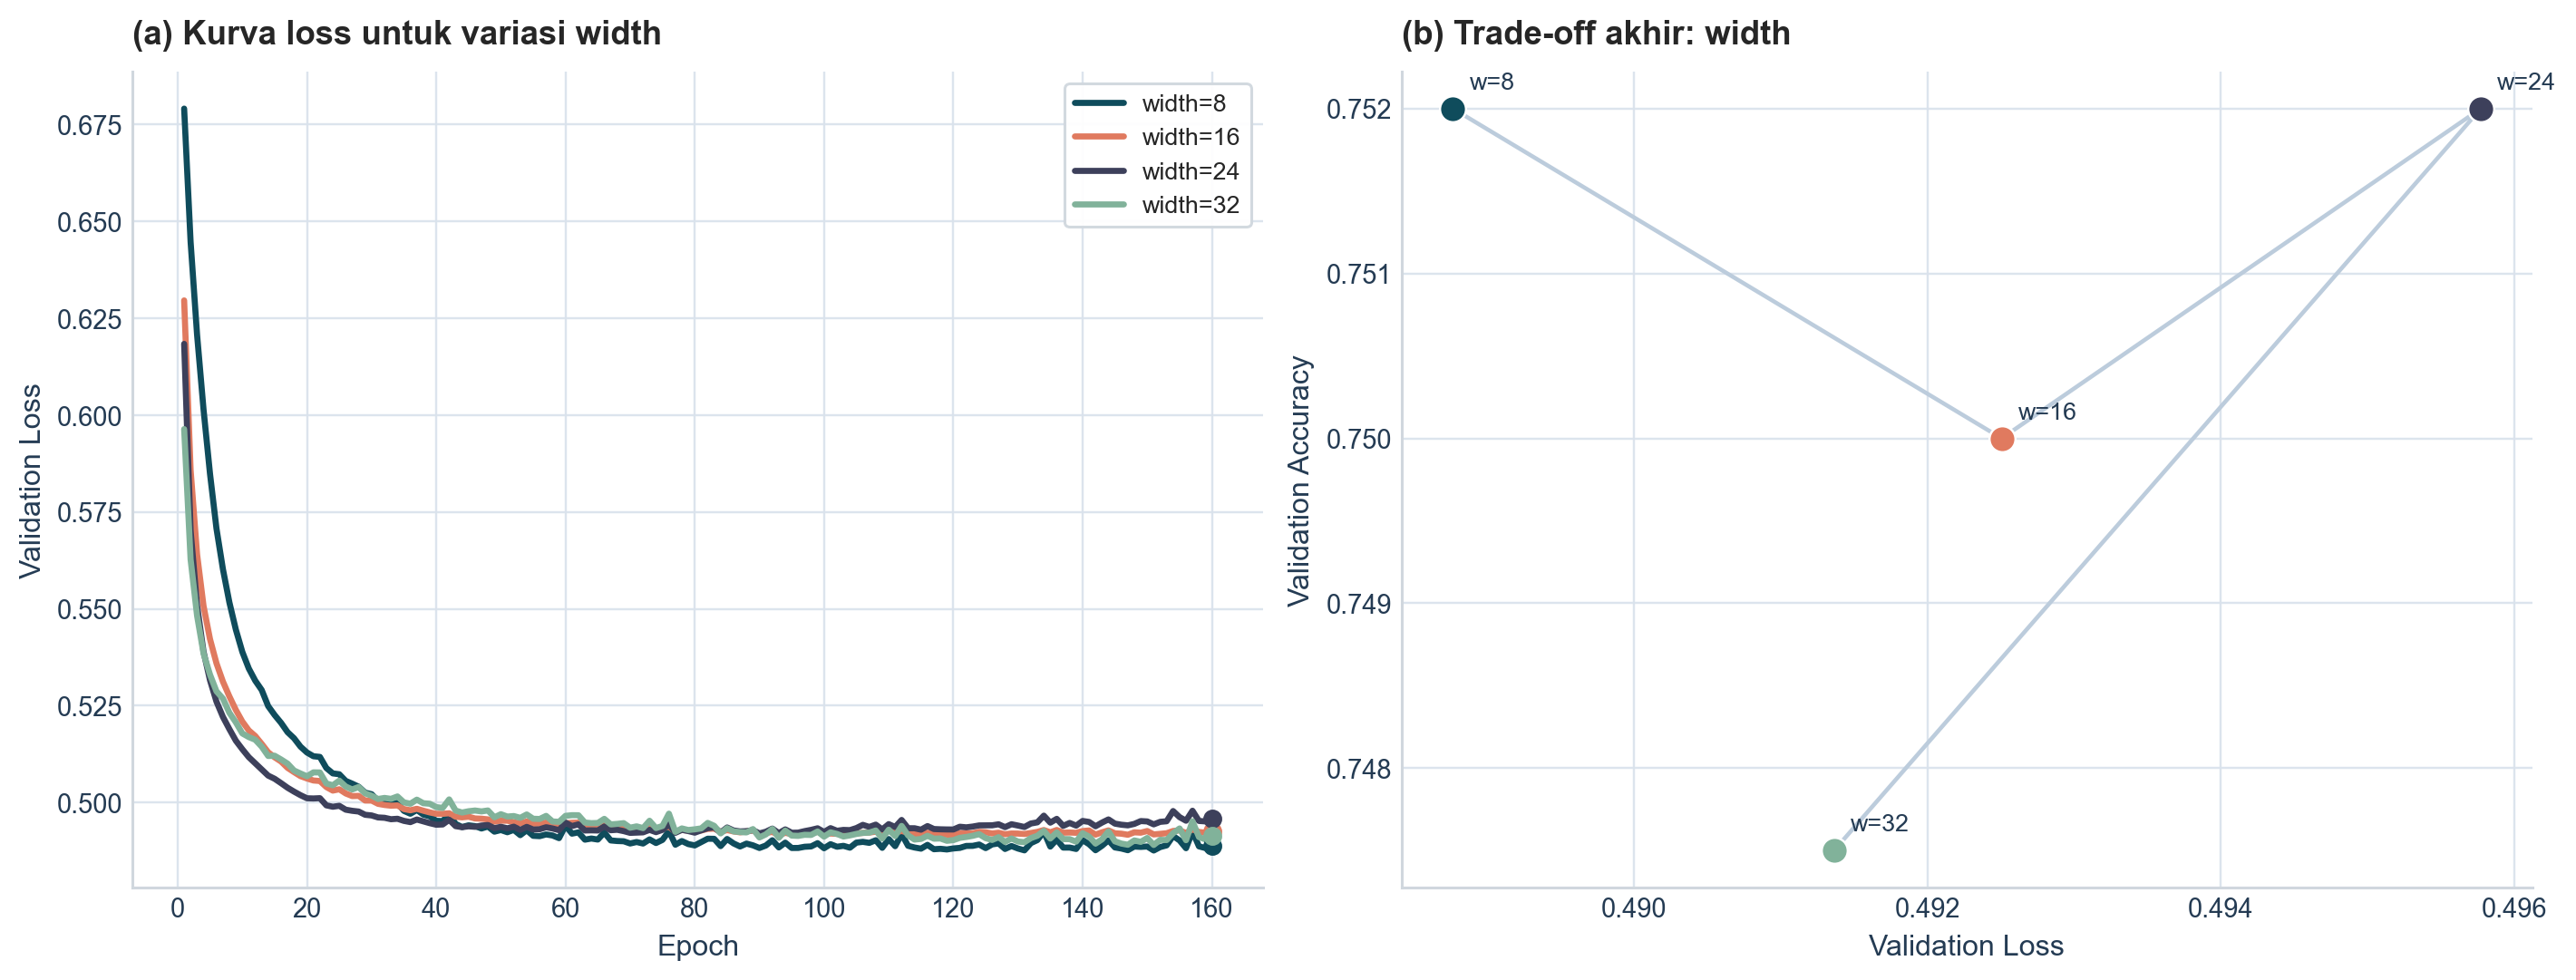
\includegraphics[width=0.98\linewidth]{figures/depth_width_width_loss.png}
\caption{Eksperimen width: panel kiri menunjukkan kurva validation loss sepanjang epoch, sedangkan panel kanan merangkum trade-off validation loss dan validation accuracy pada titik akhir pelatihan.}
\label{fig:exp-width}
\end{figure}

\begin{figure}[!tbp]
\centering
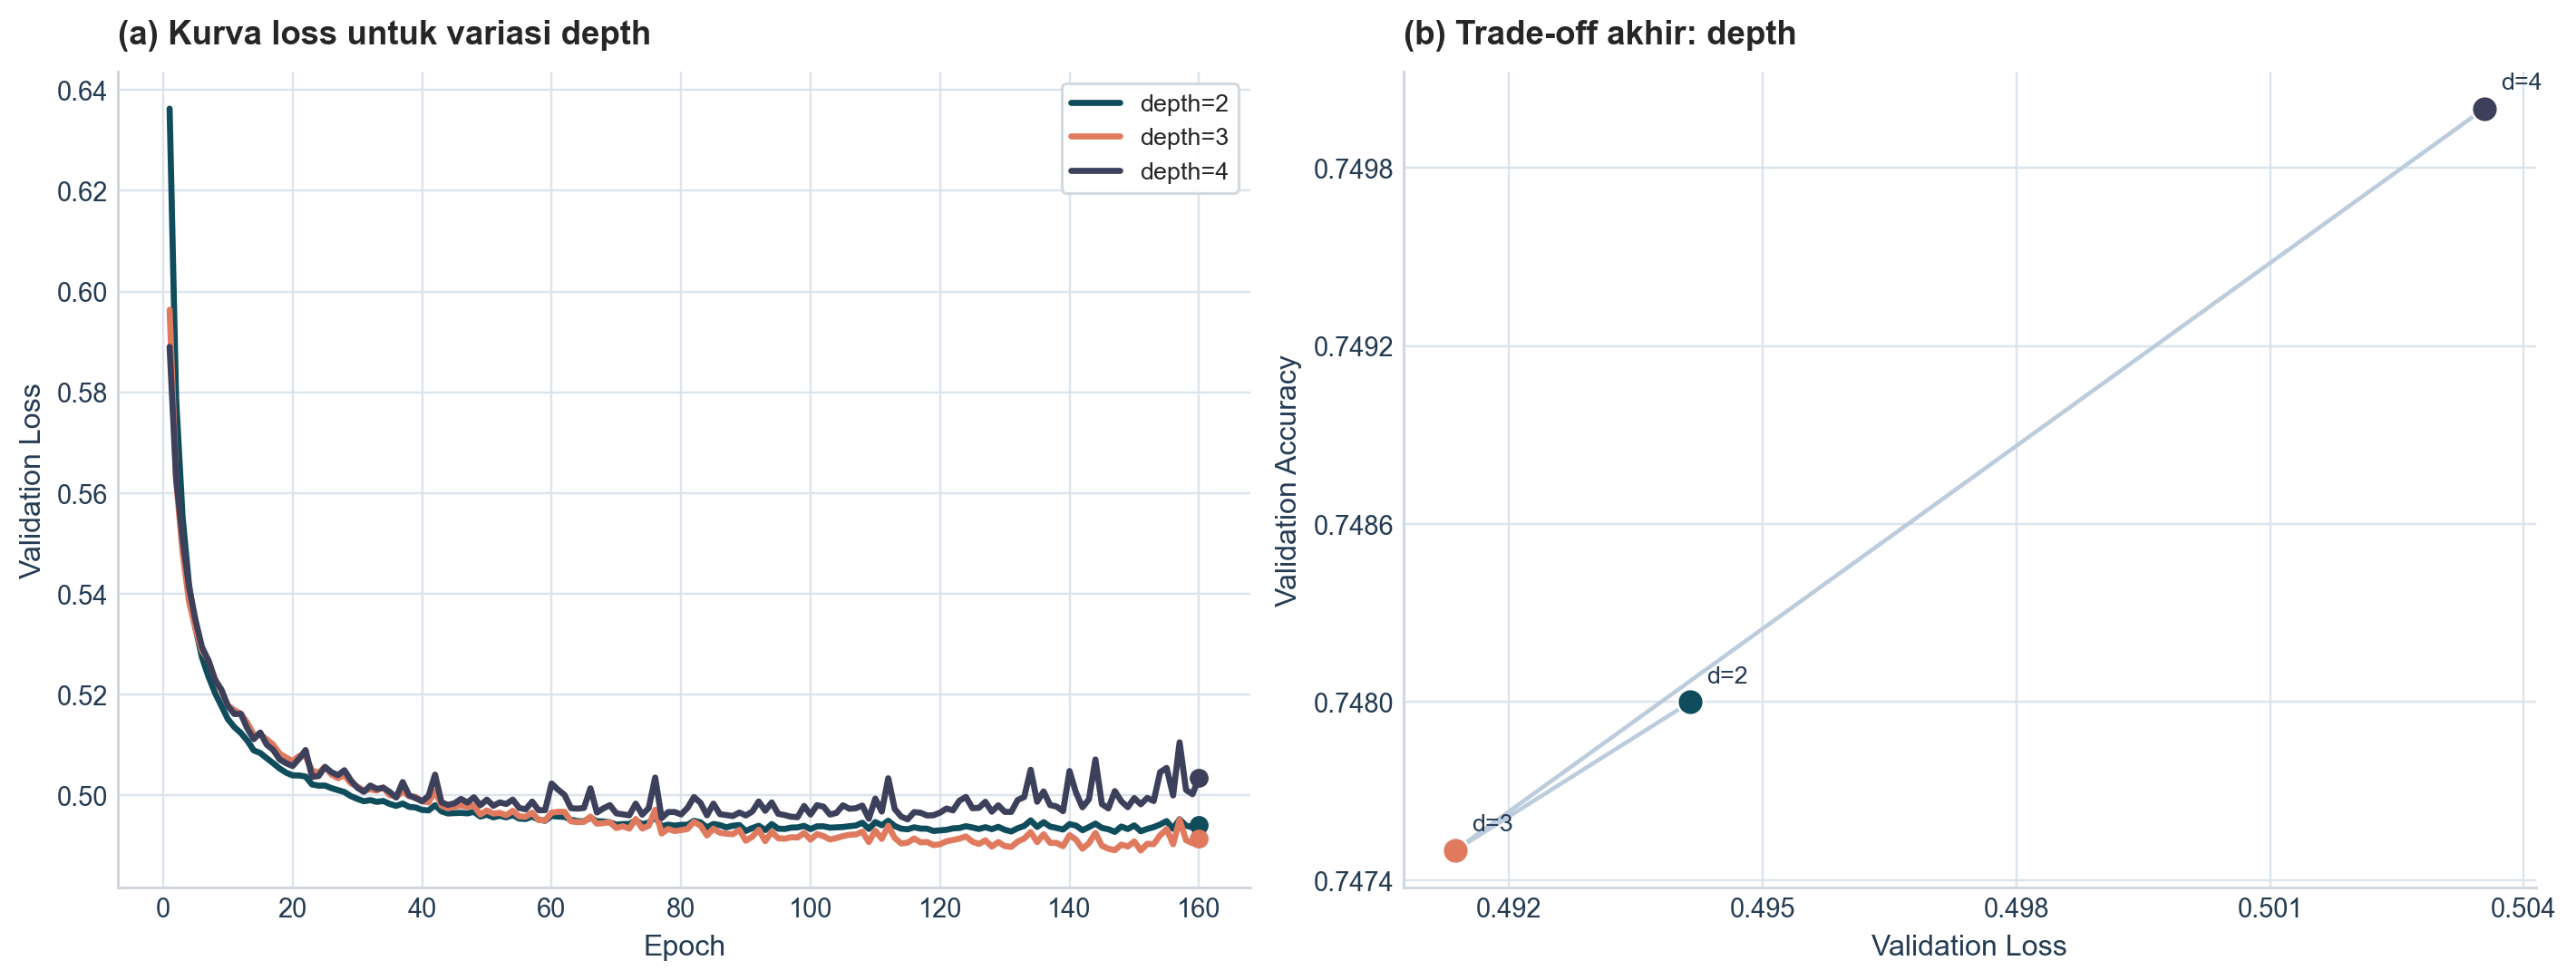
\includegraphics[width=0.98\linewidth]{figures/depth_width_depth_loss.png}
\caption{Eksperimen depth: panel kiri menunjukkan dinamika validation loss, sedangkan panel kanan menampilkan trade-off akhir antara loss dan akurasi untuk tiap kedalaman jaringan.}
\label{fig:exp-depth}
\end{figure}

\subsection{Pengaruh Fungsi Aktivasi}
Pada studi ini, arsitektur, optimizer, \textit{learning rate}, regularisasi, dan inisialisasi dibuat sama. Satu-satunya bagian yang diubah adalah fungsi aktivasi. Dengan cara ini, perbedaan hasil yang muncul lebih mudah dikaitkan ke pilihan aktivasi. Secara umum, aktivasi yang gradiennya lebih stabil biasanya membantu proses training, sedangkan aktivasi yang terlalu mudah jenuh bisa membuat optimisasi melambat. Hasil pada Gambar~\ref{fig:exp-activation-loss} dan Gambar~\ref{fig:exp-activation-dist} menunjukkan bahwa pilihan aktivasi memang memengaruhi kecepatan konvergensi dan kualitas hasil akhir. Pada run terbaru, \texttt{sigmoid} dan \texttt{selu} sama-sama memberi akurasi tertinggi 0.7535, sedangkan \texttt{sigmoid} juga memberi \textit{validation loss} terendah 0.490337. Ini menunjukkan bahwa hasil aktivasi bisa cukup dekat satu sama lain dan perubahan kecil pada setup eksperimen bisa mengubah aktivasi mana yang terlihat paling unggul.

\begin{figure}[!tbp]
\centering
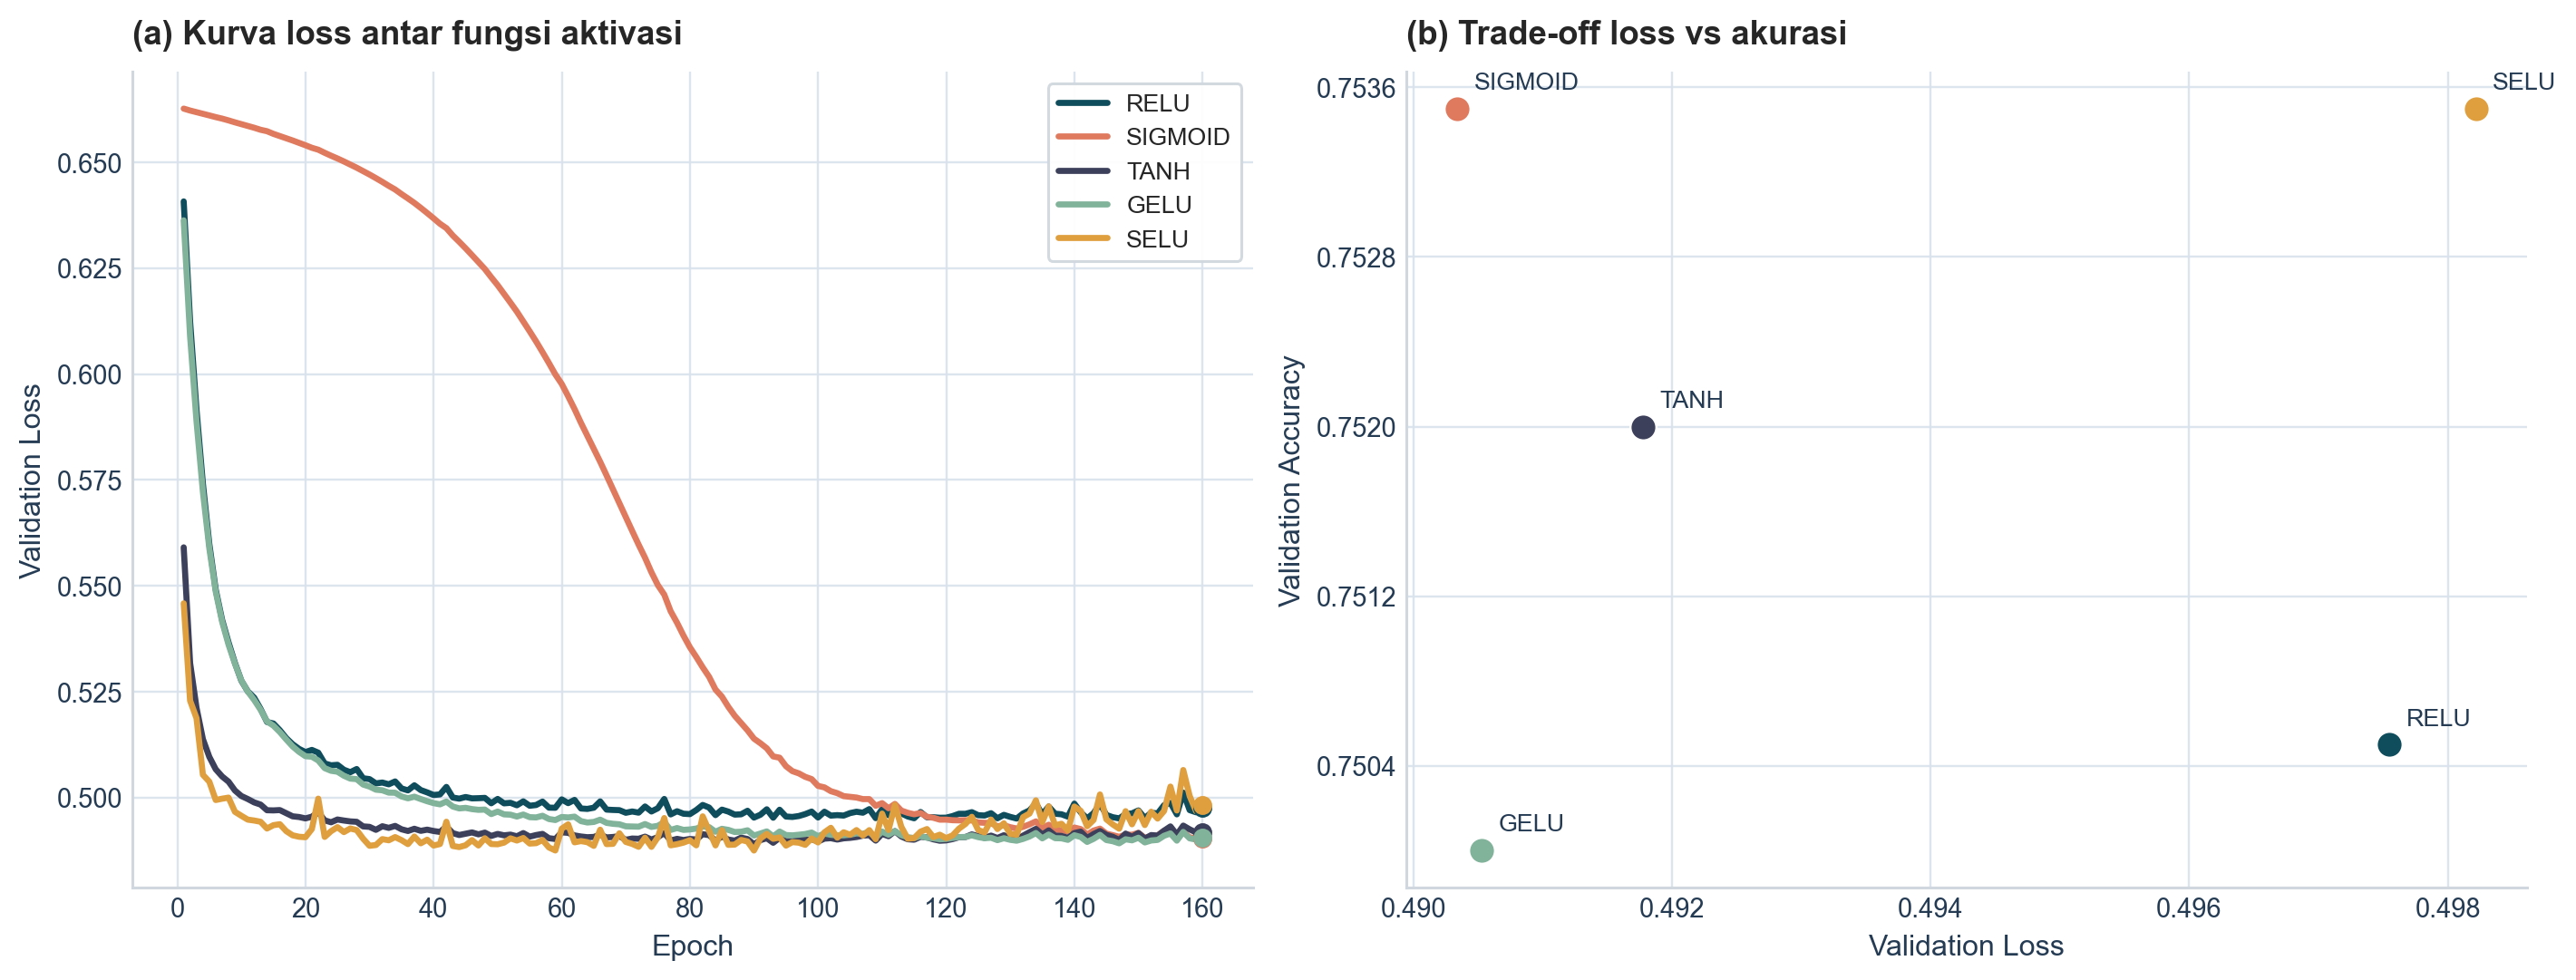
\includegraphics[width=0.98\linewidth]{figures/activation_loss.png}
\caption{Eksperimen fungsi aktivasi: panel kiri menunjukkan kurva validation loss, sedangkan panel kanan memetakan trade-off validation loss dan validation accuracy untuk setiap aktivasi.}
\label{fig:exp-activation-loss}
\end{figure}

\begin{figure}[!tbp]
\centering
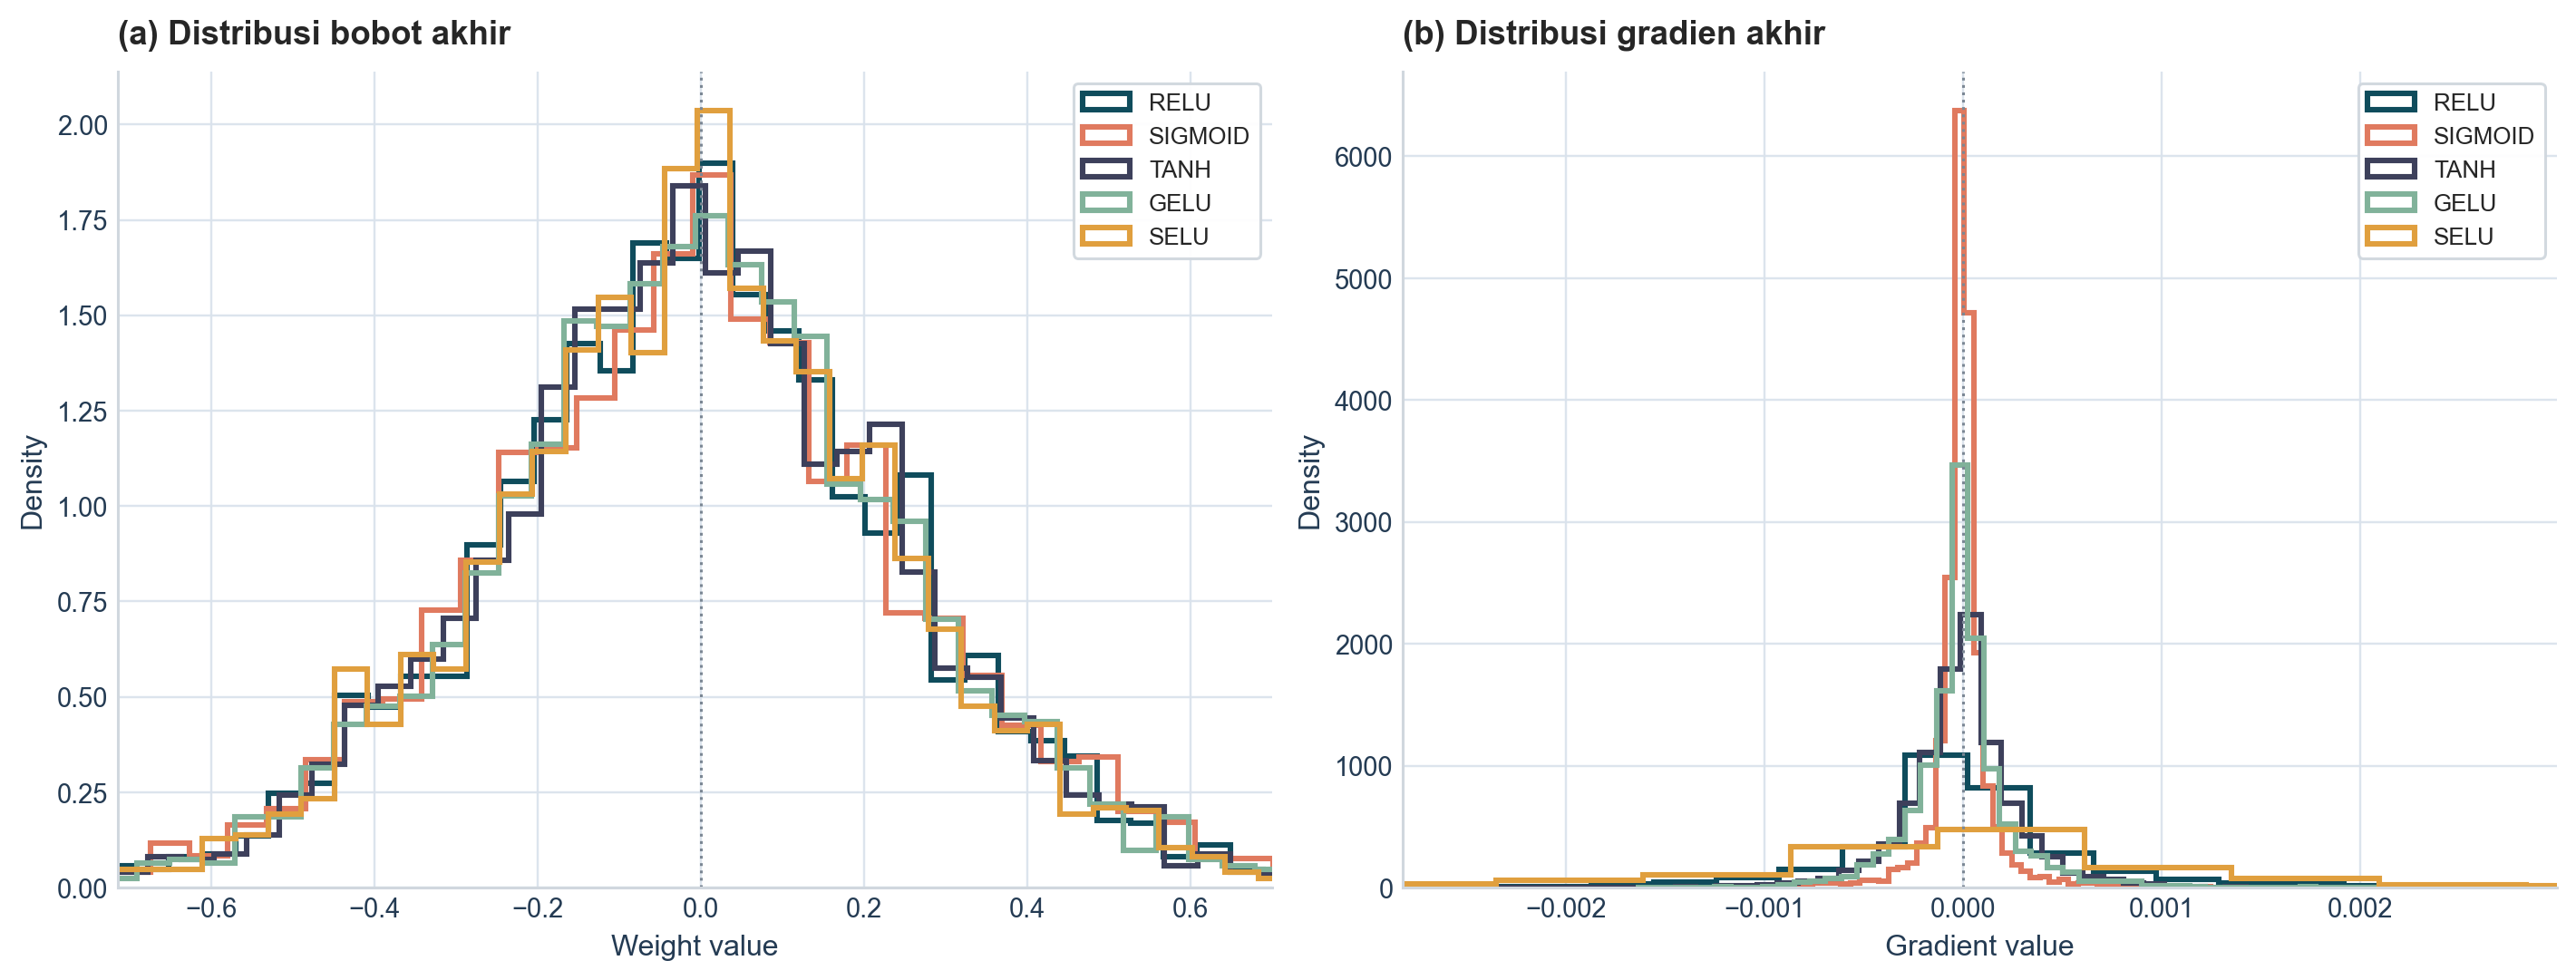
\includegraphics[width=0.98\linewidth]{figures/activation_distribution.png}
\caption{Eksperimen fungsi aktivasi: panel kiri memperlihatkan distribusi bobot akhir, sedangkan panel kanan memperlihatkan distribusi gradien akhir untuk tiap aktivasi.}
\label{fig:exp-activation-dist}
\end{figure}

\subsection{Pengaruh \textit{Learning Rate}}
\textit{Learning rate} menentukan seberapa besar langkah update yang diambil model saat training. Karena itu, eksperimen ini memakai tiga nilai yang cukup berjauhan: 0.10, 0.03, dan 0.005. Tujuannya supaya lebih jelas melihat perbedaan antara kondisi yang terlalu agresif, cukup pas, dan terlalu hati-hati. Hasil pada Gambar~\ref{fig:exp-lr} menunjukkan bahwa \textit{learning rate} besar seperti 0.10 membuat \textit{validation loss} lebih tidak stabil. Pada run terbaru, lr=0.03 memberi \textit{validation loss} terbaik 0.491365 sedangkan lr=0.005 memberi akurasi sedikit lebih tinggi, yaitu 0.7490. Dari sini terlihat bahwa pemilihan \textit{learning rate} sangat berpengaruh ke kestabilan training dan hasil akhir.

\begin{figure}[!tbp]
\centering
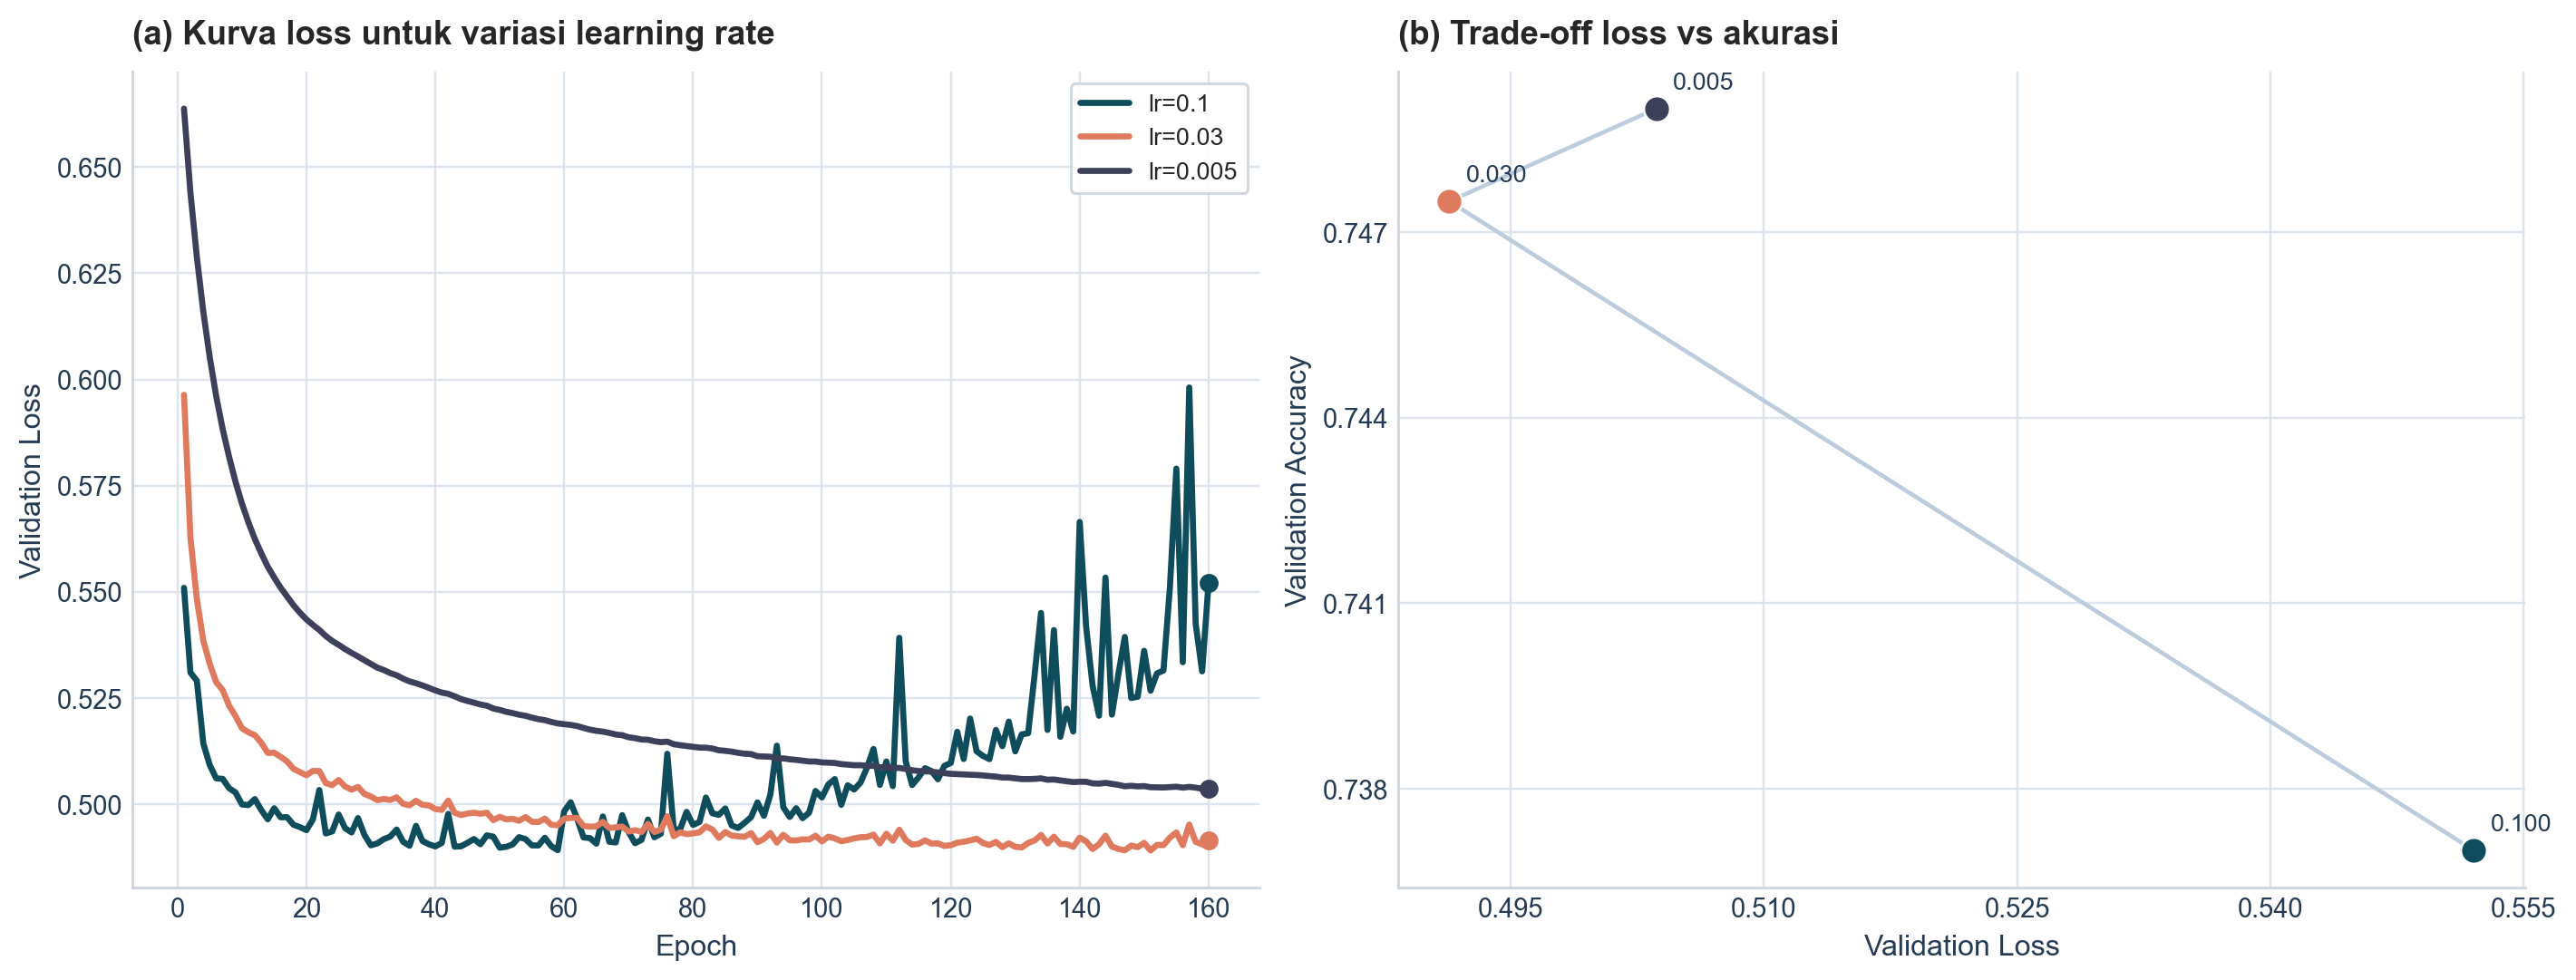
\includegraphics[width=0.98\linewidth]{figures/learning_rate_loss.png}
\caption{Eksperimen \textit{learning rate}: panel kiri menunjukkan kurva validation loss, sedangkan panel kanan merangkum trade-off antara validation loss dan validation accuracy pada akhir pelatihan.}
\label{fig:exp-lr}
\end{figure}

\subsection{Pengaruh Inisialisasi Bobot}
Eksperimen ini membandingkan tiga skema inisialisasi, yaitu \texttt{zero}, Xavier, dan He \citep{glorot2010difficulty,he2015delving}. Secara intuitif, bagian ini ingin melihat apakah pilihan nilai awal bobot benar-benar memengaruhi proses training. \texttt{Zero} dipakai sebagai kontrol negatif karena skema ini tidak memecah simetri antar neuron. Xavier dan He dipakai sebagai dua baseline yang memang dirancang supaya sinyal dan gradien tetap berada pada skala yang wajar di awal training. Hasilnya cukup jelas. Pada Gambar~\ref{fig:exp-init} dan Tabel~\ref{tab:compact_summary}, inisialisasi \texttt{zero} tertinggal jauh dari Xavier dan He. Xavier memberi hasil terbaik sedangkan He tetap jauh lebih baik daripada \texttt{zero}. Jadi, eksperimen ini menunjukkan bahwa inisialisasi bukan sekadar detail kecil. Nilai awal bobot benar-benar bisa memengaruhi apakah proses optimisasi berjalan lancar atau tidak.

\begin{figure}[!tbp]
\centering
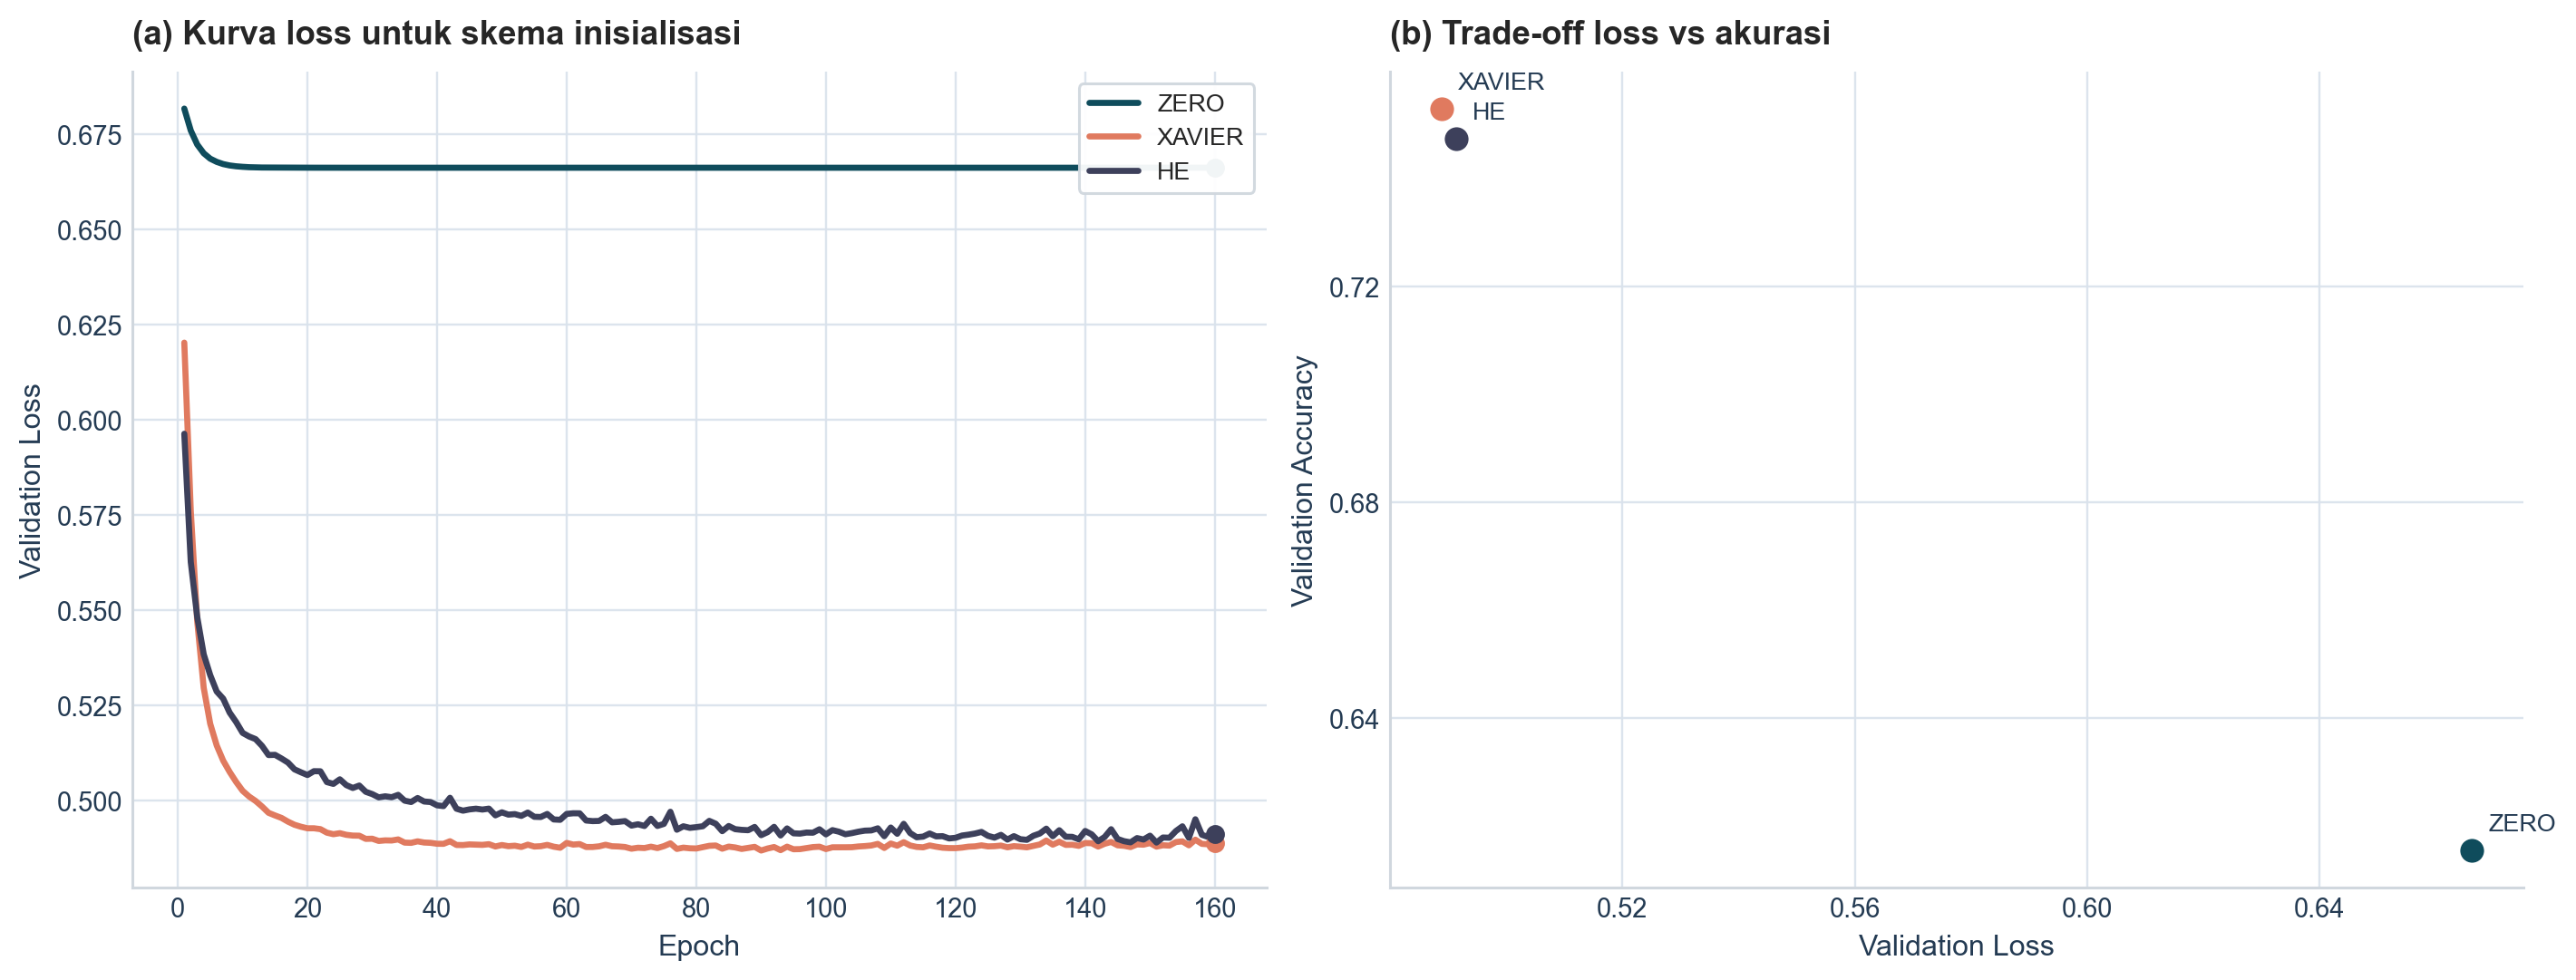
\includegraphics[width=0.98\linewidth]{figures/initialization_loss.png}
\caption{Eksperimen inisialisasi bobot: panel kiri menunjukkan kurva validation loss untuk setiap skema yang diuji, sedangkan panel kanan membandingkan trade-off akhir antara loss dan akurasi.}
\label{fig:exp-init}
\end{figure}

\subsection{Pengaruh Regularisasi}
Regularisasi diuji dalam tiga bentuk: tanpa regularisasi, L1 lemah, dan L2 lemah \citep{tibshirani1996lasso,hoerl1970ridge}. Nilai koefisiennya dipilih kecil supaya efeknya tetap bisa diamati tanpa terlalu mendominasi objective utama. Pada eksperimen ini, pengaruh regularisasi terhadap akurasi akhir memang tidak besar. Pada run terbaru, \texttt{NoReg} memberi akurasi tertinggi 0.7480 sedangkan L2 memberi \textit{validation loss} terendah 0.491365. Jadi, pada model dengan ukuran sedang seperti ini, regularisasi lebih terasa sebagai alat bantu stabilisasi daripada sumber utama peningkatan akurasi.

\begin{figure}[!tbp]
\centering
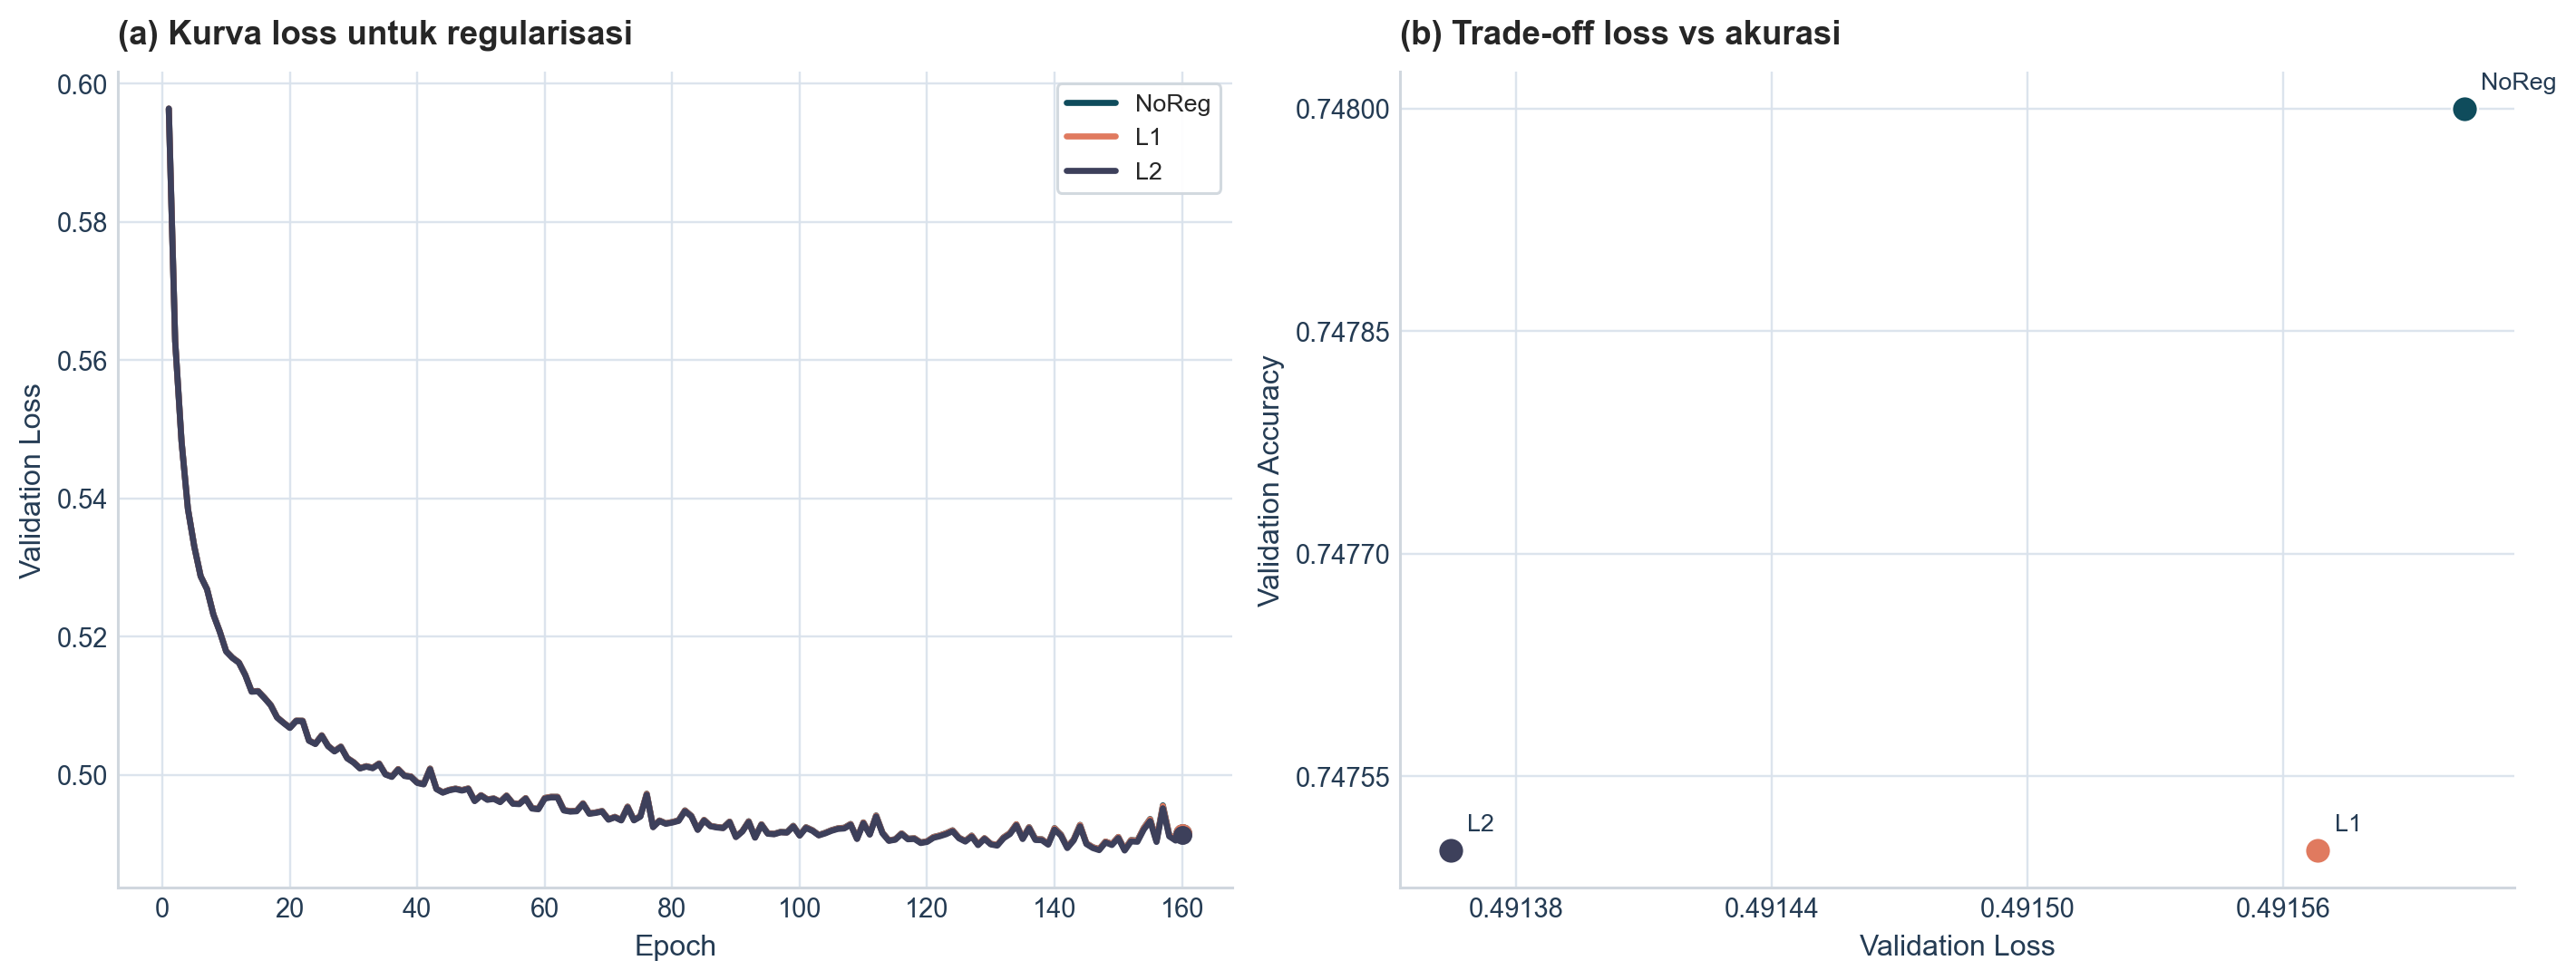
\includegraphics[width=0.98\linewidth]{figures/regularization_loss.png}
\caption{Eksperimen regularisasi: panel kiri menunjukkan kurva validation loss untuk NoReg, L1, dan L2, sedangkan panel kanan merangkum trade-off akhir antara validation loss dan validation accuracy.}
\label{fig:exp-reg-loss}
\end{figure}

\begin{figure}[!tbp]
\centering
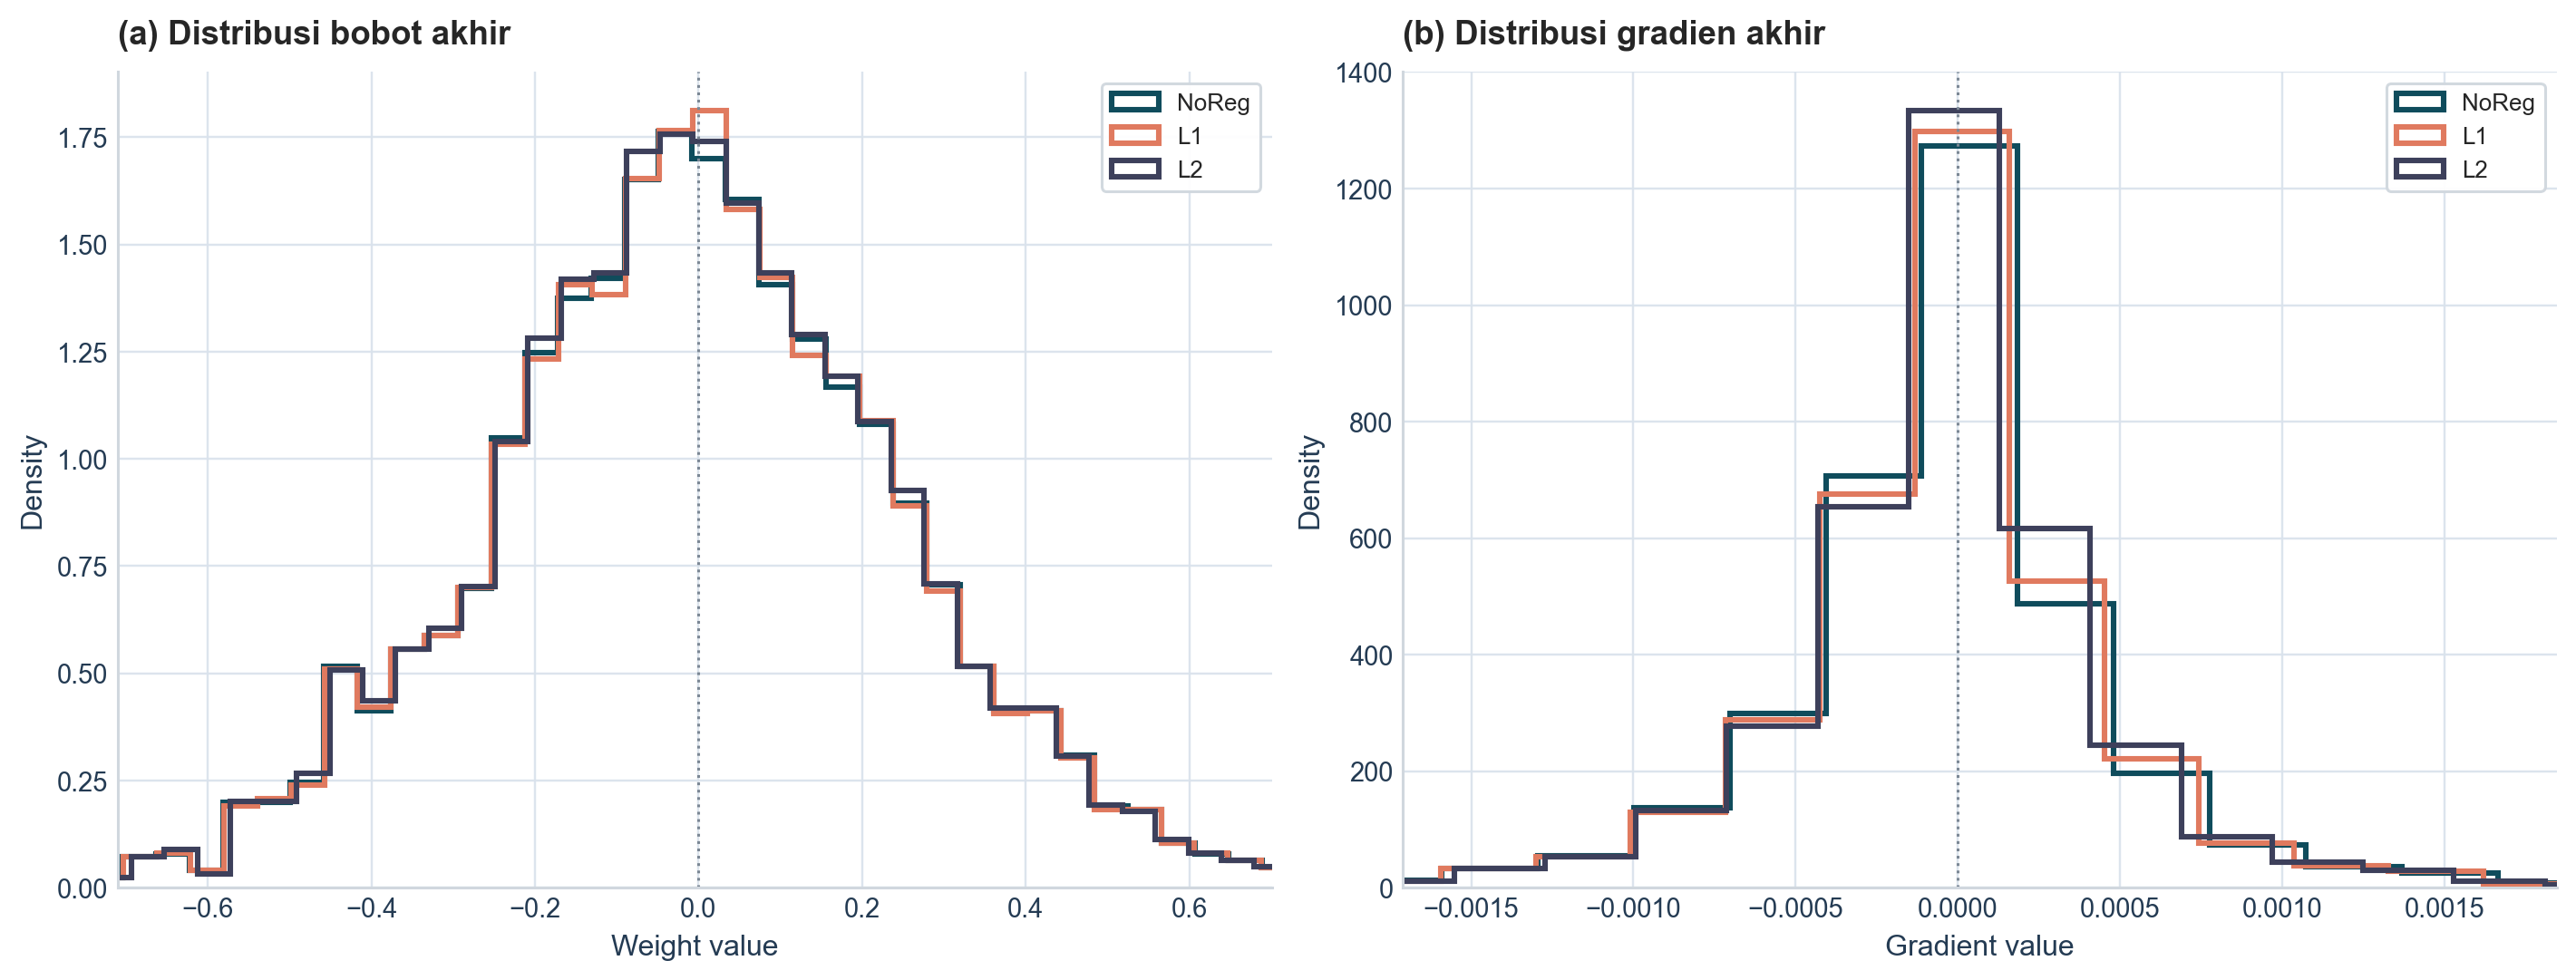
\includegraphics[width=0.98\linewidth]{figures/regularization_distribution.png}
\caption{Eksperimen regularisasi: panel kiri memperlihatkan distribusi bobot akhir, sedangkan panel kanan memperlihatkan distribusi gradien akhir setelah pelatihan.}
\label{fig:exp-reg-dist}
\end{figure}

\subsection{Pengaruh Normalisasi RMSNorm}
Eksperimen RMSNorm dibuat dengan arsitektur yang sama. Bedanya, satu model memakai RMSNorm setelah setiap transformasi linear tersembunyi sedangkan model pembanding tidak memakainya \citep{zhang2019rmsnorm,ba2016layernorm}. Dengan cara ini, pengaruh RMSNorm bisa dilihat dengan lebih jelas. Hasil pada Gambar~\ref{fig:exp-rms-loss} dan Gambar~\ref{fig:exp-rms-dist} menunjukkan bahwa RMSNorm dapat menaikkan akurasi walaupun \textit{validation loss} akhir tidak selalu ikut turun. Artinya, normalisasi ini tetap bisa membantu model membuat keputusan klasifikasi yang lebih baik pada beberapa kasus.

\begin{figure}[!tbp]
\centering
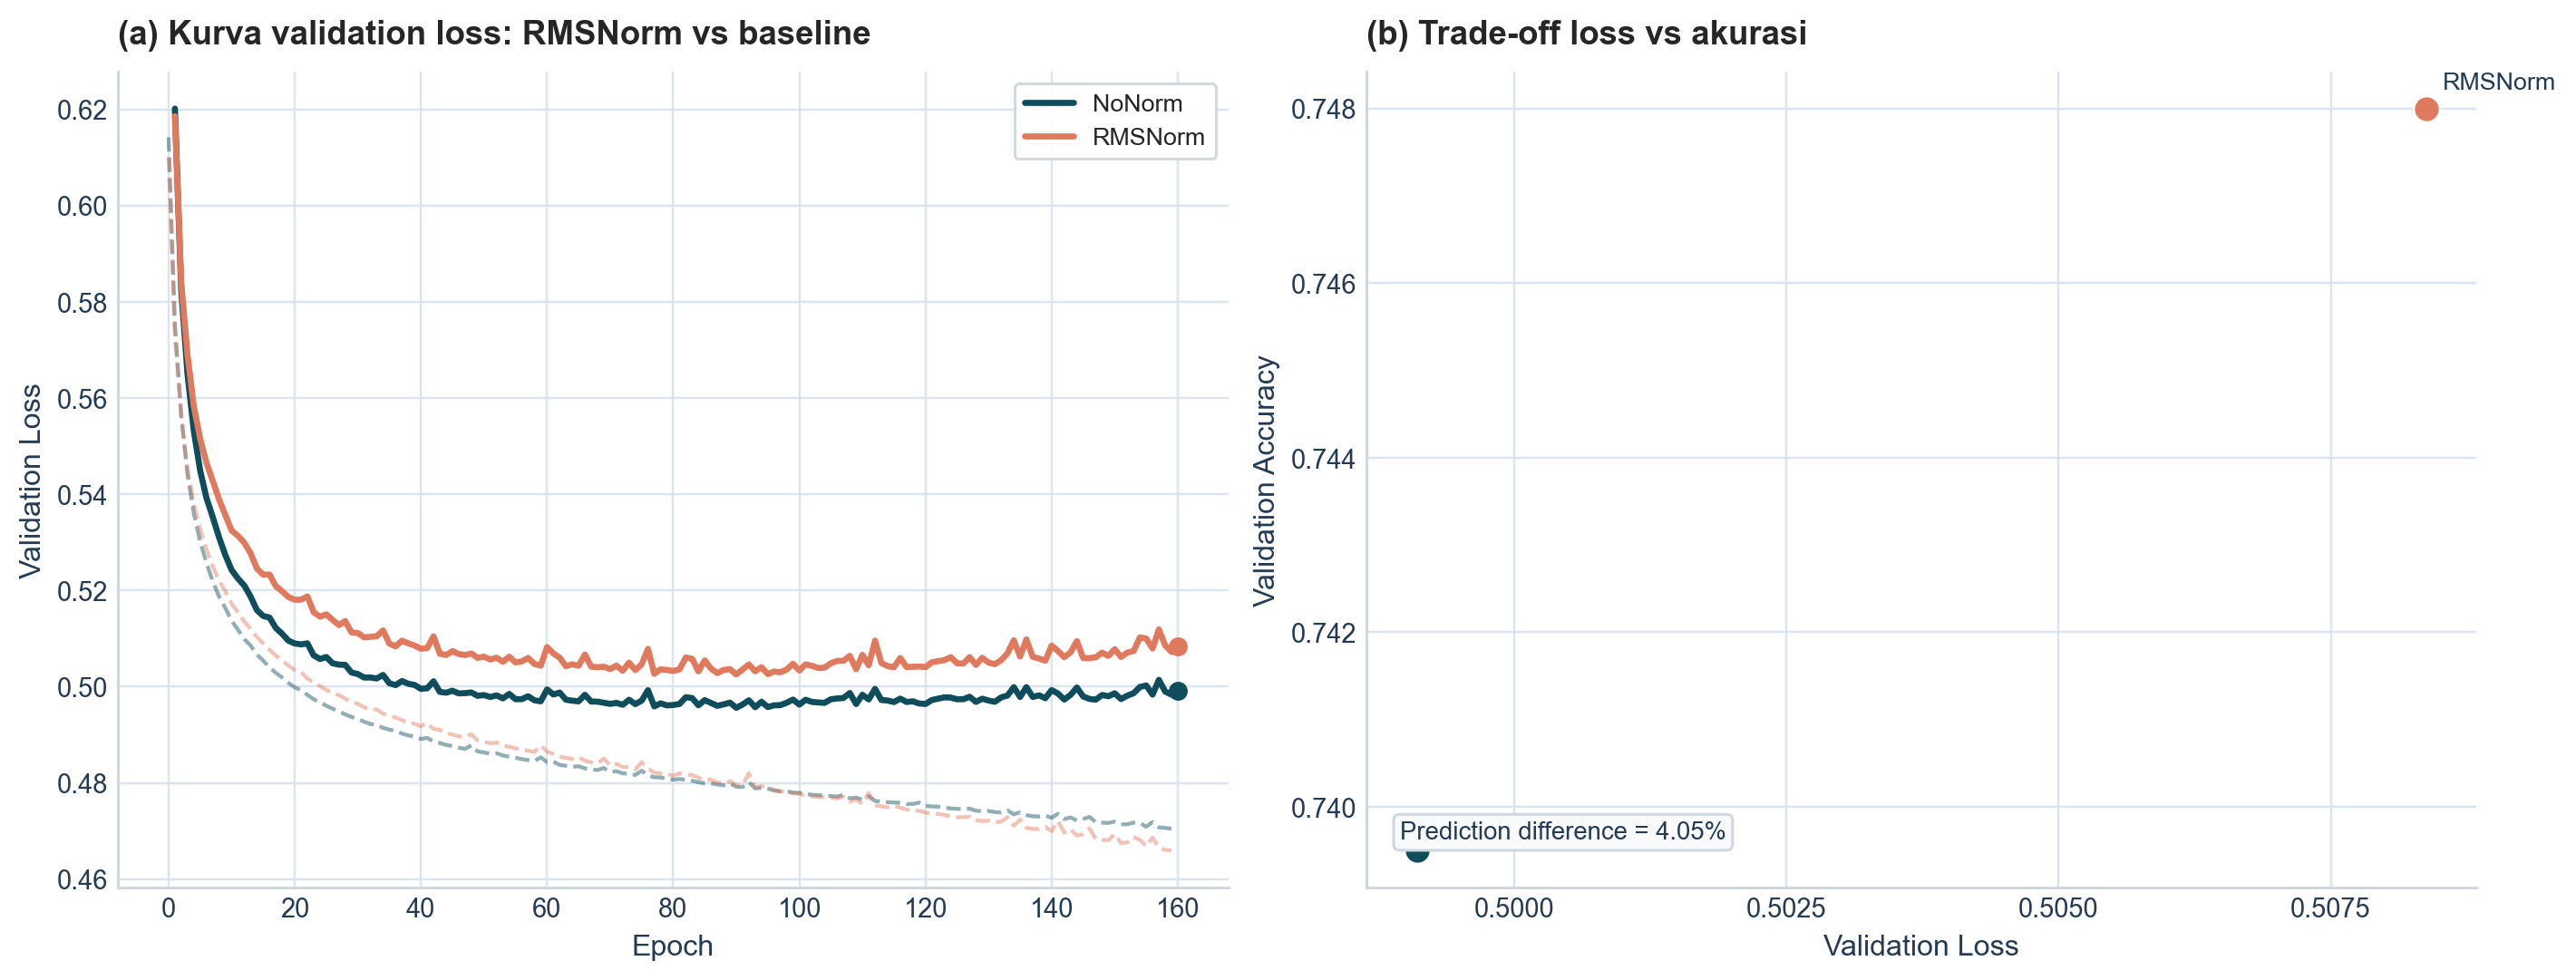
\includegraphics[width=0.98\linewidth]{figures/rmsnorm_loss.png}
\caption{Eksperimen RMSNorm: panel kiri menunjukkan kurva loss train/validasi untuk model dengan dan tanpa RMSNorm, sedangkan panel kanan merangkum trade-off akhir antara validation loss dan validation accuracy serta selisih prediksi antar model.}
\label{fig:exp-rms-loss}
\end{figure}

\begin{figure}[!tbp]
\centering
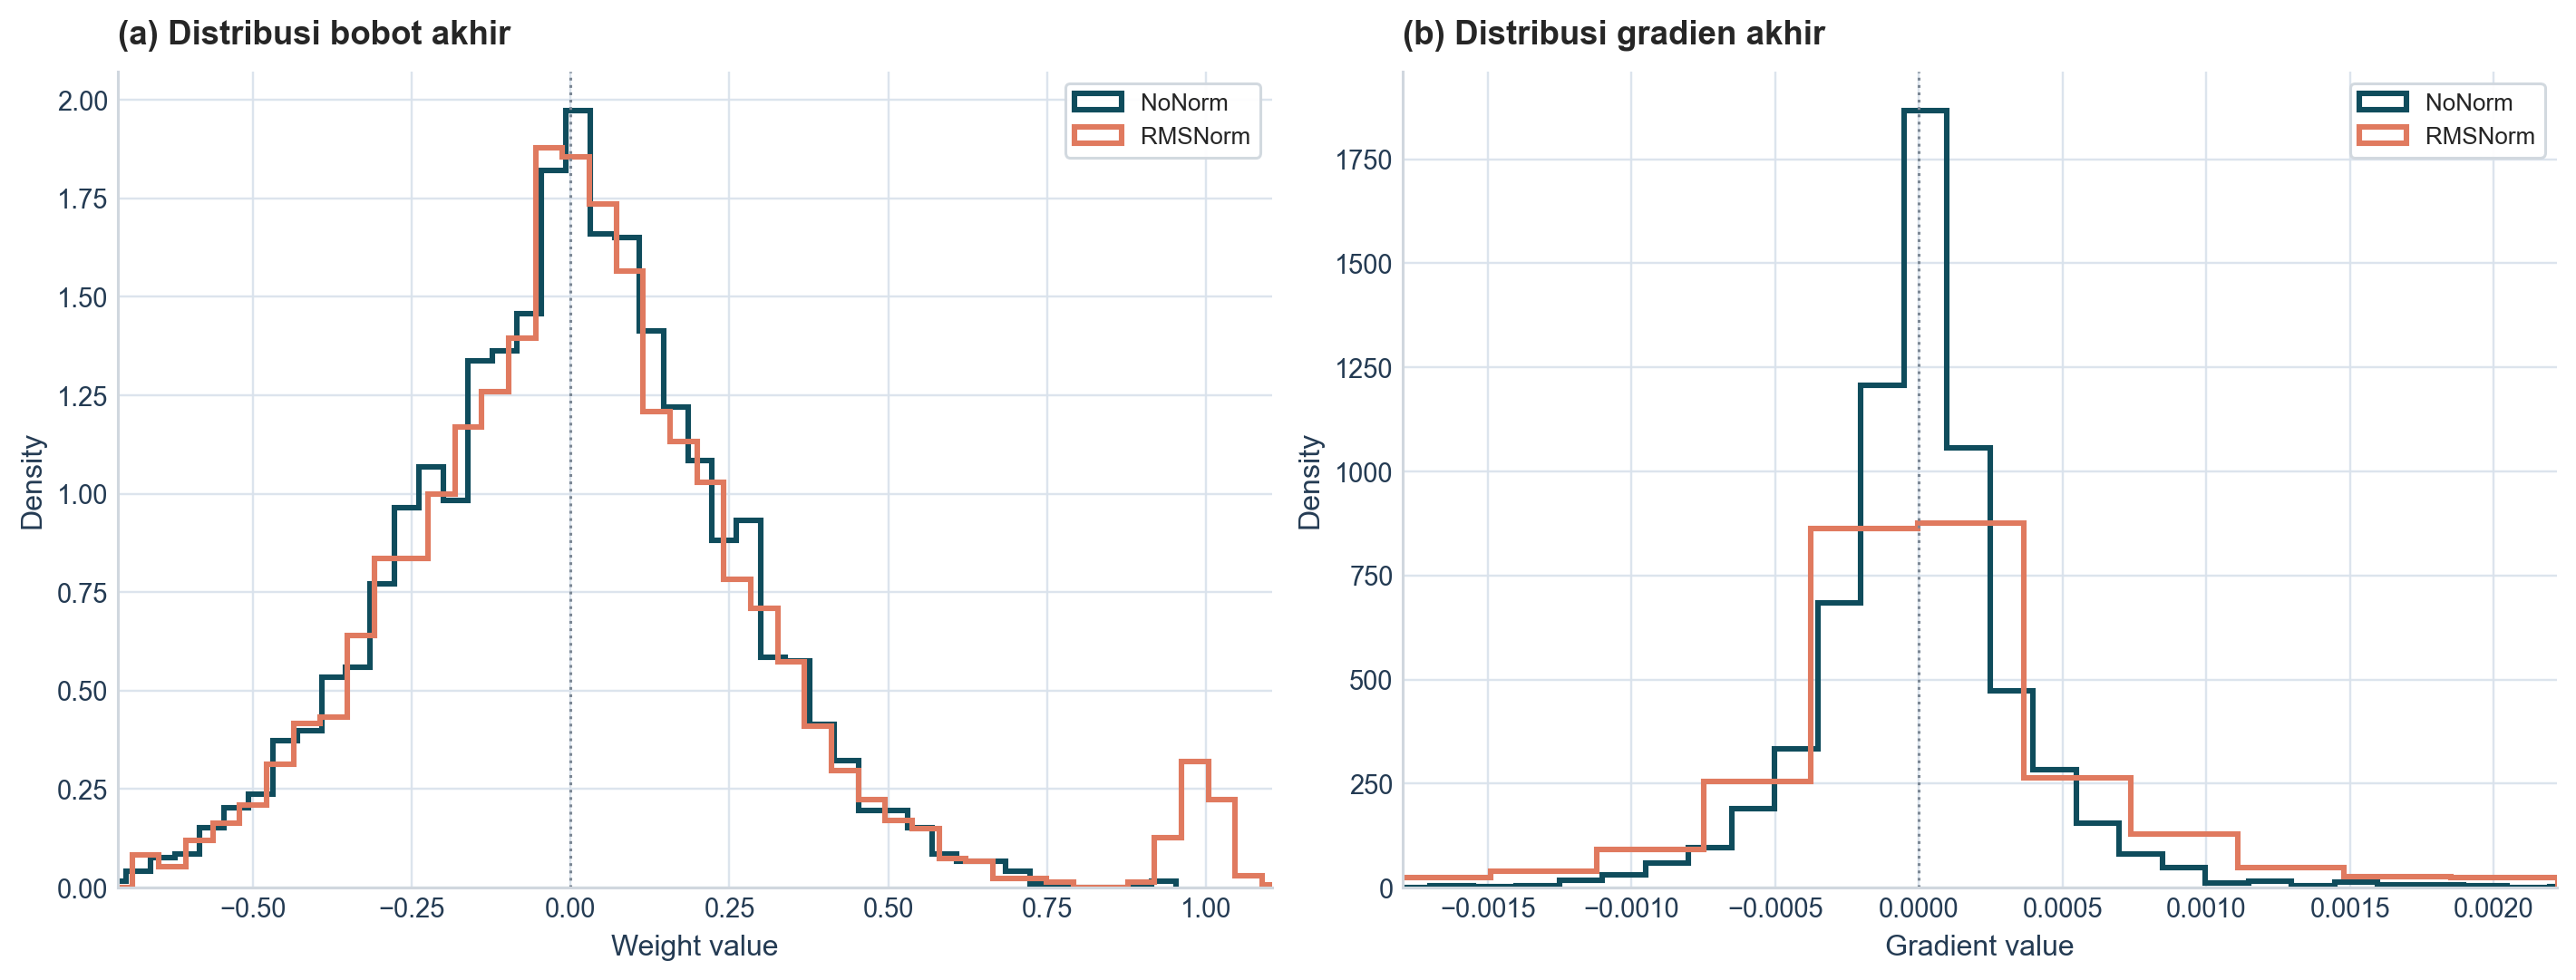
\includegraphics[width=0.98\linewidth]{figures/rmsnorm_distribution.png}
\caption{Eksperimen RMSNorm: panel kiri memperlihatkan distribusi bobot akhir, sedangkan panel kanan memperlihatkan distribusi gradien akhir untuk model baseline dan model dengan RMSNorm.}
\label{fig:exp-rms-dist}
\end{figure}

\subsection{Perbandingan dengan \texttt{sklearn} MLP}
Sebagai baseline eksternal, model \texttt{sklearn MLPClassifier} dilatih dengan konfigurasi yang dibuat semirip mungkin: tiga hidden layer berukuran 32, aktivasi \texttt{tanh}, optimizer keluarga SGD, \textit{learning rate} 0.03, regularisasi $10^{-4}$, batch size 256, horizon 160 epoch, dan seed 123 \citep{pedregosa2011sklearn,sklearn_mlpclassifier}. Aktivasi \texttt{tanh} dipilih karena tersedia secara native di kedua framework sehingga perbandingannya lebih adil. Hasil pada Gambar~\ref{fig:exp-sklearn} menunjukkan bahwa implementasi \texttt{torchlike} memberi metrik validasi yang lebih baik pada setup ini, yaitu akurasi 0.7520 dan log-loss 0.491776 dibanding \texttt{sklearn\_mlp} yang mencapai 0.6975 dan 0.768242. Ini menunjukkan bahwa implementasi \textit{from scratch} yang kami buat tetap bisa bersaing dengan baseline dari library yang sudah mapan.

\begin{figure}[!tbp]
\centering
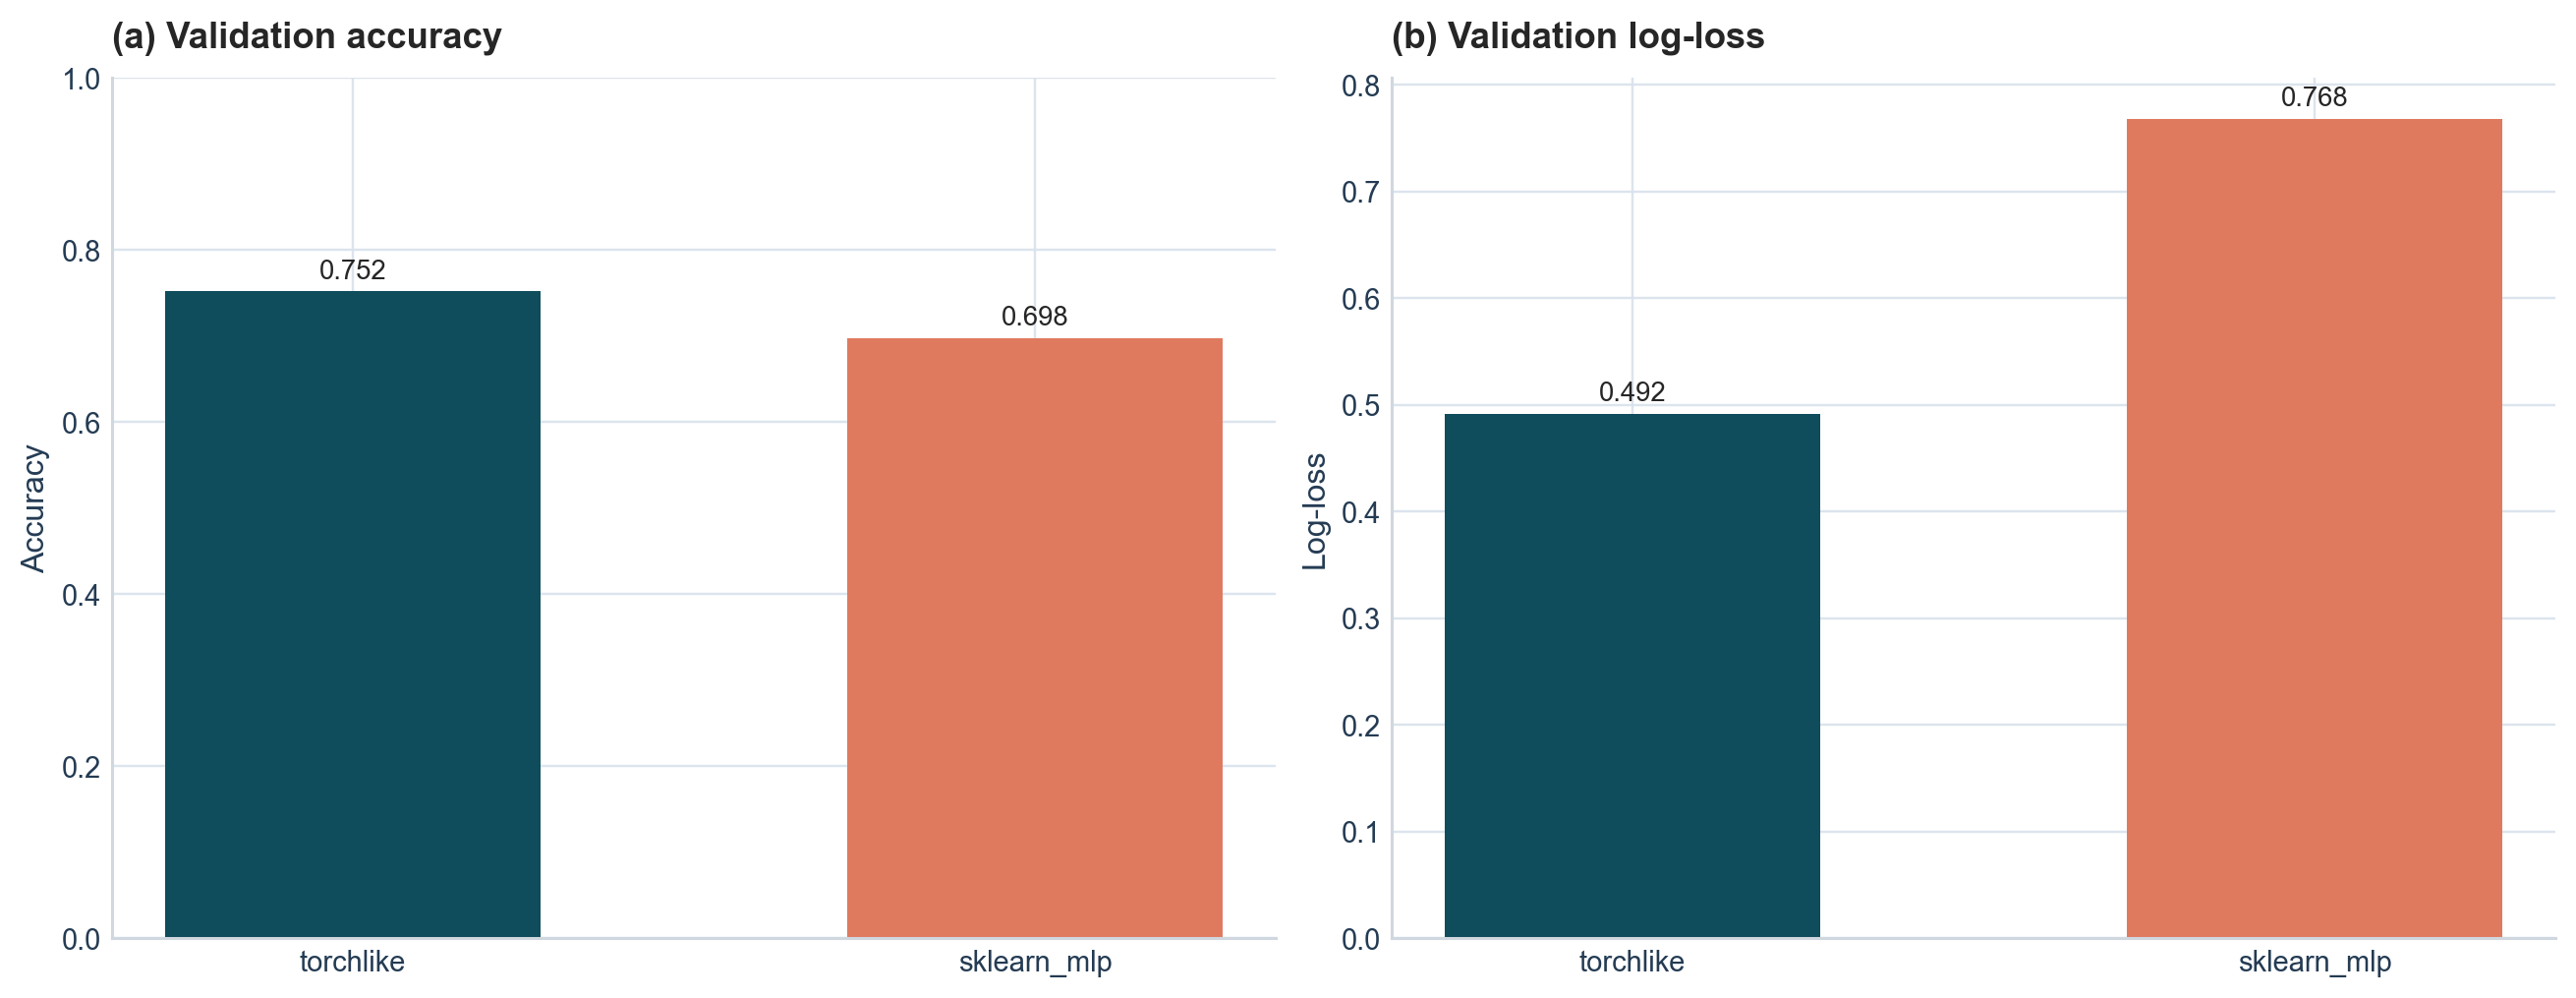
\includegraphics[width=0.9\linewidth]{figures/sklearn_comparison.png}
\caption{Perbandingan \texttt{torchlike} dan \texttt{sklearn}: panel kiri menunjukkan validation accuracy, sedangkan panel kanan menunjukkan validation log-loss.}
\label{fig:exp-sklearn}
\end{figure}

\subsection{Tambahan: SGD vs Adam}
Perbandingan optimizer dibuat pada arsitektur dasar yang sama agar yang diuji memang benar-benar cara update parameternya. \textit{Learning rate} antara SGD dan Adam tidak disamakan angkanya karena keduanya memang punya karakter langkah yang berbeda. Kalau dipaksa sama, hasilnya justru bisa bias. Karena itu, studi ini membandingkan konfigurasi yang stabil untuk masing-masing optimizer, yaitu SGD dengan 0.03 dan Adam dengan $2\times 10^{-4}$. Hasil pada Gambar~\ref{fig:exp-optimizer} menunjukkan bahwa Adam mencapai epoch terbaik lebih cepat, yaitu pada epoch 104, sedangkan SGD baru mencapai titik terbaik pada epoch 151. Namun, SGD justru memberi best loss yang lebih rendah, yaitu 0.489066, sementara Adam memberi akurasi akhir sedikit lebih tinggi, yaitu 0.7500. Jadi, pada run ini Adam unggul dari sisi kecepatan menuju titik terbaik, sedangkan SGD masih kompetitif dari sisi loss terbaik.

\begin{table}[!tbp]
\begin{center}
\small
\setlength{\tabcolsep}{4pt}
\caption{Ringkasan metrik eksperimen (compact view).}
\label{tab:compact_summary}
\begin{tabular}{llcc}
\toprule
\textbf{Kategori} & \textbf{Konfigurasi} & \textbf{Val Acc} & \textbf{Val Loss} \\
\midrule
\multirow{7}{*}{Depth/Width} & width=8 (depth=3) & 0.7520 & 0.488768 \\
 & width=16 (depth=3) & 0.7500 & 0.492507 \\
 & width=24 (depth=3) & 0.7520 & 0.495772 \\
 & width=32 (depth=3) & 0.7475 & 0.491365 \\
 & depth=2 (width=32) & 0.7480 & 0.494147 \\
 & depth=3 (width=32) & 0.7475 & 0.491365 \\
 & depth=4 (width=32) & 0.7500 & 0.503533 \\
\multirow{5}{*}{Aktivasi} & ReLU & 0.7505 & 0.497548 \\
 & Sigmoid & 0.7535 & 0.490337 \\
 & Tanh & 0.7520 & 0.491776 \\
 & GELU & 0.7500 & 0.490526 \\
 & SELU & 0.7535 & 0.498220 \\
\multirow{3}{*}{Learning Rate} & lr=0.005 & 0.7490 & 0.503617 \\
 & lr=0.03 & 0.7475 & 0.491365 \\
 & lr=0.10 & 0.7370 & 0.552049 \\
\multirow{3}{*}{Inisialisasi} & Zero & 0.6155 & 0.666224 \\
 & Xavier & 0.7530 & 0.488897 \\
 & He & 0.7475 & 0.491365 \\
\multirow{3}{*}{Regularisasi} & NoReg & 0.7480 & 0.491603 \\
 & L1 & 0.7475 & 0.491568 \\
 & L2 & 0.7475 & 0.491365 \\
\bottomrule
\end{tabular}
\end{center}
\end{table}

\begin{table}[!tbp]
\begin{center}
\small
\setlength{\tabcolsep}{4pt}
\caption{Komparasi model dan optimizer.}
\label{tab:compact_compare}
\begin{tabular}{llccc}
\toprule
\textbf{Eksperimen} & \textbf{Konfigurasi} & \textbf{Val Acc} & \textbf{Val Loss} & \textbf{Catatan} \\
\midrule
\multirow{2}{*}{RMSNorm} & SGD-NoNorm & 0.7395 & 0.499106 & baseline \\
 & SGD-RMSNorm & 0.7480 & 0.508377 & pred diff 4.05\% \\
\multirow{2}{*}{Sklearn} & torchlike & 0.7520 & 0.491776 & log-loss \\
 & sklearn\_MLP & 0.6975 & 0.768242 & log-loss \\
\multirow{2}{*}{Optimizer} & SGD & 0.7475 & 0.491365 & best 0.489066@ep151 \\
 & Adam & 0.7500 & 0.494638 & best 0.493030@ep104 \\
\bottomrule
\end{tabular}
\end{center}
\end{table}

\begin{figure}[!tbp]
\centering
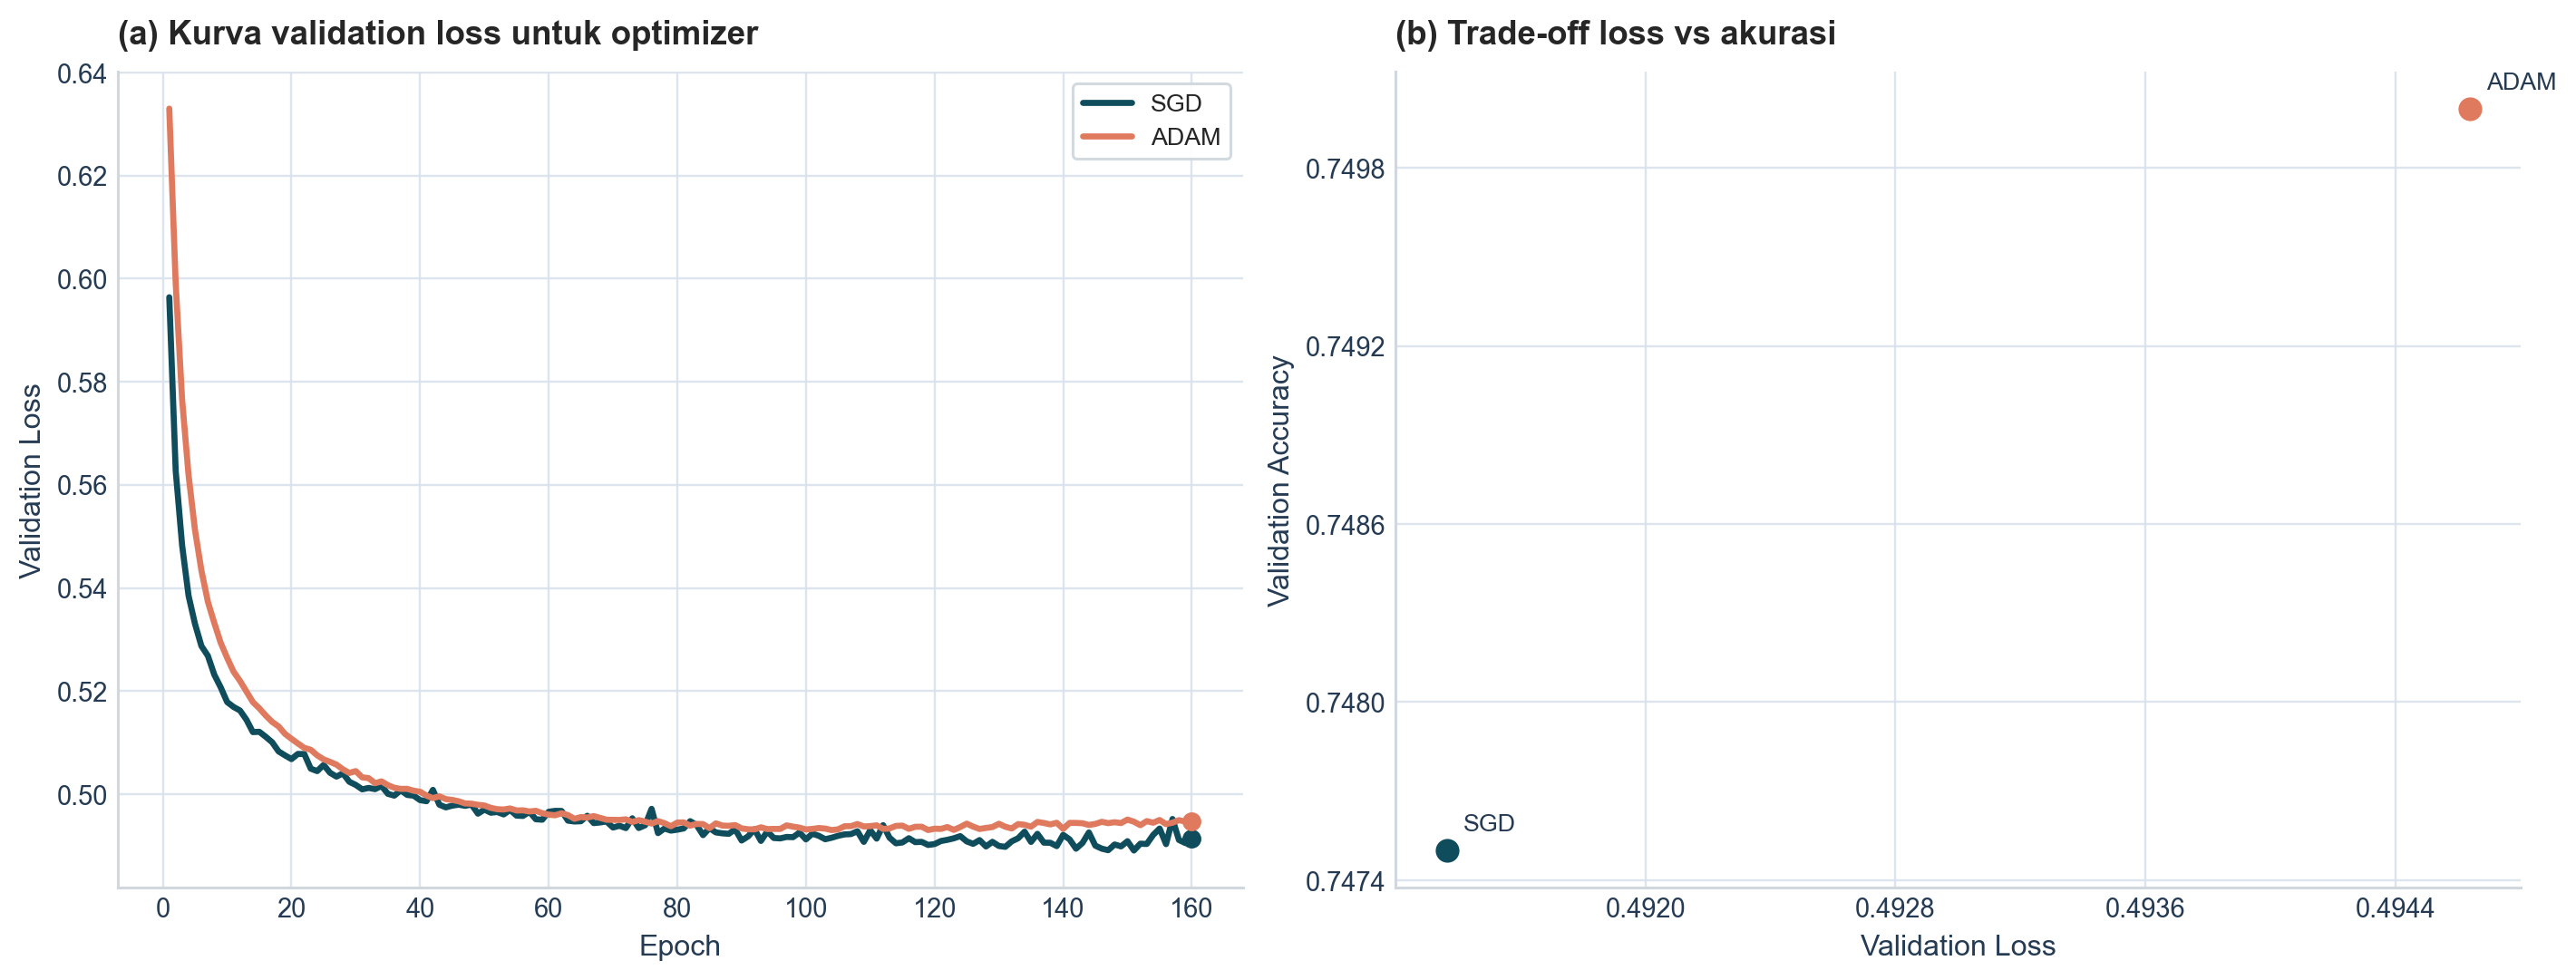
\includegraphics[width=0.98\linewidth]{figures/optimizer_loss.png}
\caption{Perbandingan optimizer: panel kiri menunjukkan kurva validation loss untuk SGD dan Adam, sedangkan panel kanan merangkum trade-off akhir antara validation loss dan validation accuracy.}
\label{fig:exp-optimizer}
\end{figure}
  
\section{Kesimpulan dan Saran}
Implementasi \texttt{torchlike} berhasil membangun pipeline pelatihan FFNN secara end-to-end mulai dari autodiff, fungsi aktivasi, inisialisasi bobot, optimizer, regularisasi, sampai RMSNorm. Dari eksperimen yang dilakukan, terlihat bahwa kapasitas model yang lebih besar tidak selalu memberi generalisasi yang lebih baik. Pilihan aktivasi dan inisialisasi juga cukup berpengaruh ke jalannya optimisasi, sedangkan RMSNorm pada beberapa kondisi bisa membantu hasil klasifikasi. Secara khusus, eksperimen inisialisasi menunjukkan bahwa \texttt{zero} bukan pilihan awal yang baik karena gagal memecah simetri, sedangkan Xavier dan He jauh lebih stabil. Untuk pengembangan selanjutnya, eksperimen bisa diulang pada beberapa seed dan ditambah metrik lain seperti \textit{confusion matrix} atau analisis kalibrasi probabilitas.

\section{Pembagian Tugas}
Pembagian tugas anggota kelompok dirangkum secara eksplisit pada Tabel~\ref{tab:kontribusi}. Ringkasan ini memetakan setiap anggota ke komponen implementasi dan rancangan eksperimen yang menjadi tanggung jawab utamanya.
\begin{table}[!tbp]
\begin{center}
\caption{Tabel kontribusi anggota kelompok \texttt{TorchIsAllYouNeed}.}
\label{tab:kontribusi}
\begin{tabularx}{\linewidth}{llX}
\toprule
\textbf{Nama} & \textbf{NIM} & \textbf{Kontribusi} \\
\midrule
Shanice Feodora Tjahjono & 13523097 & Linear, Activation Functions, Experimental Design \\
Muhammad Fathur Rizky & 13523105 & SGD, Adam, Automatic Differentiation, RMSNorm \\
Ahmad Wicaksono & 13523121 & Loss Functions, Experimental Design \\
\bottomrule
\end{tabularx}
\end{center}
\end{table}

\section{Lampiran}
\subsection{Repositori Proyek}
Kode sumber implementasi, eksperimen, dan artefak pendukung laporan tersedia pada:
\begin{center}
\url{https://github.com/fathurwithyou/TorchIsAllYouNeed}
\end{center}

\begin{thebibliography}{99}
\bibitem{goodfellow2016dl}
Ian Goodfellow, Yoshua Bengio, and Aaron Courville.
\newblock \emph{Deep Learning}.
\newblock MIT Press, 2016.

\bibitem{kingma2015adam}
Diederik P. Kingma and Jimmy Ba.
\newblock Adam: A Method for Stochastic Optimization.
\newblock In \emph{International Conference on Learning Representations (ICLR)}, 2015.

\bibitem{zhang2019rmsnorm}
Biao Zhang and Rico Sennrich.
\newblock Root Mean Square Layer Normalization.
\newblock In \emph{Advances in Neural Information Processing Systems (NeurIPS)}, 2019.

\bibitem{glorot2010difficulty}
Xavier Glorot and Yoshua Bengio.
\newblock Understanding the difficulty of training deep feedforward neural networks.
\newblock In \emph{Proceedings of the Thirteenth International Conference on Artificial Intelligence and Statistics (AISTATS)}, 2010.

\bibitem{he2015delving}
Kaiming He, Xiangyu Zhang, Shaoqing Ren, and Jian Sun.
\newblock Delving Deep into Rectifiers: Surpassing Human-Level Performance on ImageNet Classification.
\newblock In \emph{IEEE International Conference on Computer Vision (ICCV)}, 2015.

\bibitem{hendrycks2016gelu}
Dan Hendrycks and Kevin Gimpel.
\newblock Gaussian Error Linear Units (GELUs).
\newblock \emph{arXiv preprint arXiv:1606.08415}, 2016.

\bibitem{klambauer2017selfnormalizing}
Gunter Klambauer, Thomas Unterthiner, Andreas Mayr, and Sepp Hochreiter.
\newblock Self-Normalizing Neural Networks.
\newblock In \emph{Advances in Neural Information Processing Systems (NeurIPS)}, 2017.

\bibitem{nair2010relu}
Vinod Nair and Geoffrey E. Hinton.
\newblock Rectified Linear Units Improve Restricted Boltzmann Machines.
\newblock In \emph{Proceedings of the 27th International Conference on Machine Learning (ICML)}, 2010.

\bibitem{ba2016layernorm}
Jimmy Lei Ba, Jamie Ryan Kiros, and Geoffrey E. Hinton.
\newblock Layer Normalization.
\newblock \emph{arXiv preprint arXiv:1607.06450}, 2016.

\bibitem{wengert1964ad}
Robert E. Wengert.
\newblock A simple automatic derivative evaluation program.
\newblock \emph{Communications of the ACM}, 7(8):463--464, 1964.

\bibitem{linnainmaa1976taylor}
Seppo Linnainmaa.
\newblock Taylor expansion of the accumulated rounding error.
\newblock \emph{BIT Numerical Mathematics}, 16(2):146--160, 1976.

\bibitem{werbos1974thesis}
Paul J. Werbos.
\newblock \emph{Beyond Regression: New Tools for Prediction and Analysis in the Behavioral Sciences}.
\newblock PhD thesis, Harvard University, 1974.

\bibitem{rumelhart1986backprop}
David E. Rumelhart, Geoffrey E. Hinton, and Ronald J. Williams.
\newblock Learning representations by back-propagating errors.
\newblock \emph{Nature}, 323(6088):533--536, 1986.

\bibitem{baydin2018ad}
Atilim Gunes Baydin, Barak A. Pearlmutter, Alexey Andreyevich Radul, and Jeffrey Mark Siskind.
\newblock Automatic Differentiation in Machine Learning: a Survey.
\newblock \emph{Journal of Machine Learning Research}, 18(153):1--43, 2018.

\bibitem{robbins1951sa}
Herbert Robbins and Sutton Monro.
\newblock A Stochastic Approximation Method.
\newblock \emph{The Annals of Mathematical Statistics}, 22(3):400--407, 1951.

\bibitem{bottou2012tricks}
Leon Bottou.
\newblock Stochastic Gradient Descent Tricks.
\newblock In Gr\'egoire Montavon, Genevieve Orr, and Klaus-Robert Muller, editors, \emph{Neural Networks: Tricks of the Trade}, pages 421--436. Springer, 2012.

\bibitem{tibshirani1996lasso}
Robert Tibshirani.
\newblock Regression Shrinkage and Selection via the Lasso.
\newblock \emph{Journal of the Royal Statistical Society: Series B}, 58(1):267--288, 1996.

\bibitem{hoerl1970ridge}
Arthur E. Hoerl and Robert W. Kennard.
\newblock Ridge Regression: Biased Estimation for Nonorthogonal Problems.
\newblock \emph{Technometrics}, 12(1):55--67, 1970.

\bibitem{loshchilov2017adamw}
Ilya Loshchilov and Frank Hutter.
\newblock Decoupled Weight Decay Regularization.
\newblock \emph{arXiv preprint arXiv:1711.05101}, 2017.

\bibitem{paszke2019pytorch}
Adam Paszke et al.
\newblock PyTorch: An Imperative Style, High-Performance Deep Learning Library.
\newblock In \emph{Advances in Neural Information Processing Systems (NeurIPS)}, 2019.

\bibitem{pedregosa2011sklearn}
Fabian Pedregosa et al.
\newblock Scikit-learn: Machine Learning in Python.
\newblock \emph{Journal of Machine Learning Research}, 12:2825--2830, 2011.

\bibitem{pytorch_bcewithlogitsloss}
PyTorch Contributors.
\newblock BCEWithLogitsLoss documentation.
\newblock PyTorch documentation. Available at \url{https://pytorch.org/docs/stable/generated/torch.nn.BCEWithLogitsLoss.html}. Accessed March 6, 2026.

\bibitem{sklearn_standardscaler}
scikit-learn Contributors.
\newblock StandardScaler documentation.
\newblock scikit-learn documentation. Available at \url{https://scikit-learn.org/stable/modules/generated/sklearn.preprocessing.StandardScaler.html}. Accessed March 6, 2026.

\bibitem{sklearn_onehotencoder}
scikit-learn Contributors.
\newblock OneHotEncoder documentation.
\newblock scikit-learn documentation. Available at \url{https://scikit-learn.org/stable/modules/generated/sklearn.preprocessing.OneHotEncoder.html}. Accessed March 6, 2026.

\bibitem{sklearn_mlpclassifier}
scikit-learn Contributors.
\newblock MLPClassifier documentation.
\newblock scikit-learn documentation. Available at \url{https://scikit-learn.org/stable/modules/generated/sklearn.neural_network.MLPClassifier.html}. Accessed March 6, 2026.

\bibitem{bartlett2006convexity}
Peter~L. Bartlett, Michael~I. Jordan, and Jon~D. McAuliffe.
\newblock Convexity, Classification, and Risk Bounds.
\newblock \emph{Journal of the American Statistical Association}, 101(473):138--156, 2006.
\end{thebibliography}

\end{document}
